%%
%% Journal of Systems and Software submission
%% Built from the cas-dc (double column) Elsevier template.
%%
\documentclass[a4paper,fleqn]{cas-dc}

\usepackage[authoryear,longnamesfirst]{natbib}

% Ensure any Computer Modern fallback glyphs (e.g. accented author names in
% the bibliography) use scalable Latin Modern Type1 outlines instead of
% triggering on-the-fly Metafont bitmap generation.
\usepackage{lmodern}

% ---------------------------------------------------------------------------
% Additional packages needed for figures, algorithms and code listings.
% (graphicx, amsmath/amsfonts/amssymb, booktabs, multirow, array, colortbl,
%  xcolor and hyperref are already loaded by cas-dc.cls.)
% ---------------------------------------------------------------------------
\usepackage{bm}
\usepackage{pifont}
\newcommand{\ymark}{\ding{51}}
\newcommand{\xmark}{\ding{55}}

\usepackage{tikz}
\usetikzlibrary{arrows.meta,positioning,calc,fit,backgrounds,shapes.geometric,decorations.pathreplacing}
\usepackage{pgfplots}
\pgfplotsset{compat=1.18}
\definecolor{heatblue}{RGB}{33,113,181}
\newcommand{\CTcs}{0.85}
\newcommand{\EXcs}{0.78}

\usepackage[ruled,vlined]{algorithm2e}
\usepackage{listings}
\lstdefinestyle{codebox}{
  frame=single,
  numbers=left,
  numberstyle=\tiny\color{gray},
  basicstyle=\ttfamily\scriptsize,
  columns=fullflexible,
  breaklines=true,
  keepspaces=true,
  keywordstyle=\color{blue!70}\bfseries,
  commentstyle=\color{green!50!black}\itshape,
  stringstyle=\color{orange!80!black},
}
\lstdefinestyle{errorbox}{
  frame=single,
  basicstyle=\ttfamily\scriptsize,
  backgroundcolor=\color{red!6},
  columns=fullflexible,
  breaklines=true,
  keepspaces=true,
}
\lstdefinestyle{taskbox}{
  frame=single,
  basicstyle=\ttfamily\scriptsize,
  backgroundcolor=\color{blue!4},
  columns=fullflexible,
  breaklines=true,
  keepspaces=true,
}
\lstdefinelanguage{Rust}{
  keywords={fn,let,mut,if,for,in,return,true,false,struct,impl,
             pub,use,mod,where,match,enum,loop,while,break,self},
  sensitive=true,
  morecomment=[l]{//},
  morecomment=[s]{/*}{*/},
  morestring=[b]",
}

\graphicspath{{figs/}}

\begin{document}
\let\WriteBookmarks\relax
\def\floatpagepagefraction{1}
\def\textpagefraction{.001}

% Short title
\shorttitle{GMM-Router for Continual Code Generation}

% Short author
\shortauthors{Tran An Khanh}

% Main title of the paper
\title[mode=title]{GMM-Router: Density-Based Task-Agnostic Routing for Continual Code Generation}

% First author
\author[1]{Tran An Khanh}
\cormark[1]
\ead{TODO@example.edu} % TODO: insert corresponding author email
\credit{Conceptualization, Methodology, Software, Data curation, Investigation, Writing -- original draft}

\affiliation[1]{organization={School of Information and Communication Technology, Hanoi University of Science and Technology},
            addressline={TODO}, % TODO: insert street address
            city={Hanoi},
            postcode={TODO}, % TODO: insert postcode
            state={},
            country={Vietnam}}

\cortext[1]{Corresponding author}

% Here goes the abstract
\begin{abstract}
Code language models deployed in practice must adapt continuously to new programming languages, task types, and coding standards, which gives rise to continual learning for code generation: a model is trained on a sequence of tasks but risks catastrophic forgetting of earlier ones. Existing approaches rely on parameter regularization, prompt tuning, or data replay, each of which struggles with structurally diverse task streams, offers limited expressive capacity, or raises data-retention concerns. This paper studies whether routing can avoid these limitations without task identity at inference. We propose GMM-Router, which trains a task-specific low-rank adaptation (LoRA) expert per task while a diagonal Gaussian Mixture Model (GMM), fitted by Expectation-Maximization over frozen, orthonormally projected backbone representations, provides task-agnostic scores that merge expert adapters via a temperature-scaled softmax. For executable code generation, an iterative refinement stage fits a second GMM on runtime error tracebacks and combines it with the instruction router through a Jensen--Shannon-divergence-gated rule to re-predict samples that fail on the first attempt. GMM-Router is evaluated on two complementary benchmarks: an eight-task extension of CodeTask-CL scored by text-overlap metrics, and a nine-language executable benchmark scored by unit-test execution. On the diverse CodeTask sequence, GMM-Router attains the highest average score (51.62\%) among all task-agnostic baselines, with near-zero backward transfer ($-1.01\%$). On the executable benchmark, it reaches 34.40\% Pass@1 and the highest Pass@5 (47.75\%) among all evaluated methods. These results indicate that combining architectural expert isolation with density-based probabilistic routing is an effective, practical strategy for task-agnostic continual code generation.
\end{abstract}

% Research highlights
\begin{highlights}
\item GMM-Router routes inputs to per-task LoRA experts via frozen-backbone GMM scores.
\item A fixed orthonormal projection keeps the routing space stable as tasks accumulate.
\item Highest score (51.62\%) among task-agnostic methods on an 8-task CodeTask benchmark.
\item Highest Pass@5 (47.75\%) on a 9-language executable code generation benchmark.
\item JSD-gated traceback routing recovers samples that fail every Round-1 candidate.
\end{highlights}

% Keywords
\begin{keywords}
continual learning \sep code generation \sep parameter-efficient fine-tuning \sep Gaussian mixture model \sep mixture of experts \sep catastrophic forgetting \sep large language models for code
\end{keywords}

\maketitle

\section{Introduction}
\label{sec:introduction}

Large language models for code have shown strong results on a wide range of software engineering tasks, including code generation from natural language, cross-language translation, code summarization, bug repair, and program synthesis \citep{wang2021codet5,roziere2023codellama,hui2024qwen25coder,lozhkov2024starcoder2,lu2021codexglue,chen2021evaluating,austin2021program}. These results come mainly from large-scale offline training, in which data for all target tasks is collected in advance, combined into one corpus, and used to train the model over many iterations. This approach works well when the target task distribution is fixed, but it becomes harder to sustain as the number of tasks grows and deployment conditions change.

In long-term deployment, a code assistant cannot remain unchanged after its initial training. New programming languages emerge, existing frameworks change, and the range of capabilities expected of the model keeps growing. Retraining the model from scratch after each change is slow and inflexible, and in many business settings re-using old training data raises privacy concerns that limit approaches based on storing or replaying historical data. A more practical alternative lets the model absorb new tasks one at a time while continuing to handle previously learned tasks without access to old data. Standard supervised learning is not suited to this setting because it assumes the full training set is available at once and that the task distribution is stationary; neither assumption holds when a model is updated incrementally under storage or privacy constraints.

Continual learning studies exactly this problem: a model learns from a stream of tasks without forgetting what it has already learned \citep{parisi2019continual,delange2021continual}. Updates that reduce the loss on the current task tend to overwrite knowledge from earlier tasks, a phenomenon known as catastrophic forgetting \citep{mccloskey1989catastrophic,goodfellow2013empirical}. The code domain makes this problem particularly difficult because tasks vary widely in input format, output format, programming language, and evaluation criterion --- a task sequence may move from English-to-Java generation to Java-to-C\# translation, Ruby summarization, and multilingual executable program synthesis, a level of diversity comparable to the CodeTask-CL benchmark \citep{yadav2023exploring}. Existing continual learning approaches have clear limitations in this setting. Regularization methods \citep{kirkpatrick2017overcoming,zenke2017continual,aljundi2018memory} accumulate importance weights across tasks, but their penalty becomes unreliable on long and structurally diverse sequences. Prompt-based methods \citep{wang2022learning,razdaibiedina2023progressive} keep the backbone frozen but have limited representational capacity for tasks as different as translation, summarization, and repair. Sequential low-rank adaptation methods \citep{wang2023orthogonal,wang2025continual,qian2025treelora} cause destructive interference within a shared low-rank subspace; orthogonality constraints reduce but do not eliminate this problem, and the number of available orthogonal directions shrinks as tasks accumulate.

A further limitation shared by most existing approaches is the assumption that task identity is available at inference time. Methods that drop this assumption typically rely on heuristics such as nearest-centroid assignment, which break down when task embeddings overlap --- a common occurrence in code generation, where problems from different languages can produce nearly identical instruction embeddings. Current evaluation practice compounds these gaps: the most widely used continual learning benchmark for code \citep{yadav2023exploring} covers only four tasks and is scored with text-similarity metrics such as BLEU \citep{papineni2002bleu} and CodeBLEU \citep{ren2020codebleu}, which cannot detect code that looks plausible but fails functionally, and short task sequences hide long-range forgetting effects. Few prior studies combine sequential learning with executable, multilingual, unit-test-based evaluation \citep{chen2021evaluating,cassano2023multipl}.

This paper addresses task-agnostic, parameter-efficient continual learning for sequential code generation. We adopt a routing-based approach that combines per-task expert isolation with a learned probabilistic model for task identification at inference time, avoiding data replay, parameter interference, and the requirement for explicit task labels. The contributions of this paper are as follows.

\begin{enumerate}[leftmargin=*]
\item \textbf{A two-track evaluation platform for continual code generation.} We extend CodeTask-CL \citep{yadav2023exploring} with four additional tasks covering new programming languages and task types, producing a longer, more diverse eight-task sequence scored by text-overlap metrics. We additionally build a nine-language executable benchmark from OSS-Instruct, McEval-Instruct, McEval, MBPP, and MultiPL-E \citep{wei2023magicoder,chai2024mceval,austin2021program,cassano2023multipl}, in which generated programs are evaluated by running them against unit tests.
\item \textbf{A deduplication pipeline for the executable benchmark} that combines exact matching via normalized SHA-256 hashing with a near-duplicate detection stage based on shingling, MinHash, Locality-Sensitive Hashing, and exact Jaccard scoring \citep{jaccard1901distribution,broder1997resemblance,indyk1998approximate}, reducing train--test leakage.
\item \textbf{A systematic empirical comparison} of regularization-based, prompt-based, low-rank-adaptation-based, and online continual learning baselines on sequential programming tasks under a consistent training and evaluation protocol.
\item \textbf{GMM-Router}, a routing-based continual learning framework that trains a task-specific LoRA expert per task on a frozen backbone, fits a diagonal Gaussian Mixture Model by Expectation-Maximization on routing embeddings extracted through a fixed orthonormal projection, and merges expert adapters at the weight level using temperature-scaled softmax routing weights. For executable code generation, the framework further incorporates a traceback-based router that uses runtime failure signals to guide a second inference round.
\end{enumerate}

We evaluate GMM-Router against seven continual learning baselines and a task-identity upper bound on both benchmark tracks. On the diverse CodeTask benchmark, GMM-Router achieves the highest average score (51.62\%) among all task-agnostic methods, approaching the upper bound (54.15\%) with near-zero forgetting. On the executable benchmark, it achieves 34.40\% Pass@1 and the highest Pass@5 (47.75\%) among all methods evaluated.

The remainder of this paper is organized as follows. Section~\ref{sec:background} presents the motivation and the conceptual background needed to follow the proposed method. Section~\ref{sec:data} describes the data collection, formatting, and deduplication pipeline underlying the two benchmark tracks. Section~\ref{sec:methodology} presents the GMM-Router methodology. Section~\ref{sec:evaluation} defines the research questions and the experimental configuration. Section~\ref{sec:results} reports and discusses the experimental results. Section~\ref{sec:related_work} situates GMM-Router within the continual learning and mixture-of-experts literature. Section~\ref{sec:conclusion} concludes the paper and outlines directions for future work.

\section{Motivation and Background}
\label{sec:background}

\subsection{Motivation}
\label{sec:motivation}

A code assistant deployed for an extended period is rarely trained once and left unchanged. New programming languages and frameworks appear, task requirements shift, and the range of requests a model must handle keeps expanding. Two constraints make this update problem hard in practice. First, full retraining on the union of all data seen so far is computationally expensive and grows more so as the task stream lengthens. Second, data from earlier tasks --- proprietary code, private repositories, or controlled benchmark collections --- may become unavailable or unusable for retraining because of storage or privacy constraints. A practical solution must therefore let the model absorb each new task using only that task's data, while retaining acceptable performance on every task learned previously, and it must do so without knowing in advance which task an incoming request belongs to.

This paper treats sequential code generation as a case study for this problem because the tasks that a code assistant is asked to perform are structurally heterogeneous: some map natural language to code, some map code to code, and some map code to natural language, across many programming languages and syntactic conventions. This heterogeneity means that a continual learning method effective for narrow, homogeneous task streams --- as is common in image classification benchmarks --- does not automatically transfer to code. The remainder of this section introduces the concepts needed to state the problem precisely and to follow the GMM-Router methodology in Section~\ref{sec:methodology}: code language models as the pretrained backbones used throughout this study (Section~\ref{sec:clm_background}), the continual learning problem formulation (Section~\ref{sec:cl_background}), parameter-efficient fine-tuning as the adaptation mechanism (Section~\ref{sec:peft_background}), and Gaussian Mixture Models as the probabilistic tool used for routing (Section~\ref{sec:gmm_background}). Detailed comparison with prior continual learning and routing methods is deferred to Section~\ref{sec:related_work}.

\subsection{Code language models}
\label{sec:clm_background}

Large language models pretrained on source code follow one of two broad architectural families. Encoder-decoder models use a bidirectional encoder together with a causal decoder and are well suited to tasks such as translation and summarization, as in CodeT5 \citep{wang2021codet5} and CodeT5+ \citep{wang2023codet5plus}. Decoder-only models use a single stack of causal self-attention layers that processes both the input and the generated output, which is more natural for open-ended generation and completion; this family includes Code Llama \citep{roziere2023codellama}, StarCoder2 \citep{lozhkov2024starcoder2}, and Qwen2.5-Coder \citep{hui2024qwen25coder}. All of these families are built on the Transformer architecture \citep{vaswani2017attention}. Qwen2.5-Coder, a decoder-only model built for code generation, completion, reasoning, and repair, serves as the backbone throughout this paper (Section~\ref{sec:setup}). Model architecture matters for continual learning because a model updated repeatedly over time must preserve both its representations and its generation abilities across a growing task sequence; this consideration motivates keeping the backbone frozen and confining task-specific updates to a small set of parameters, as described next.

\subsection{Continual learning}
\label{sec:cl_background}

Continual learning --- also called lifelong or sequential learning --- is a setting in which a model is trained on a stream of tasks that arrive one at a time \citep{parisi2019continual,delange2021continual}. Let $\mathcal{T}_1,\ldots,\mathcal{T}_K$ denote a sequence of tasks, each associated with a training dataset
\begin{equation}
    \mathcal{D}_k = \bigl\{(x_i^{(k)},\, y_i^{(k)})\bigr\}_{i=1}^{N_k},
    \label{eq:dataset}
\end{equation}
where $x_i^{(k)}$ is an input prompt and $y_i^{(k)}$ is the target output sequence. The naive sequential update minimizes the current task loss starting from the previous parameters $\theta_{k-1}$: $\theta_k = \arg\min_{\theta}\mathbb{E}_{(x,y)\sim\mathcal{D}_k}[\ell(f_\theta(x),y)]$. This update is simple but typically causes catastrophic forgetting \citep{mccloskey1989catastrophic,kirkpatrick2017overcoming}: updates that reduce loss on the current task overwrite parameters that encoded earlier-task knowledge. In code generation, a model may lose Java-to-C\# translation ability after fine-tuning on Ruby summarization, or degrade on Python generation after adapting to Rust. An effective continual learner must balance stability (retaining earlier tasks) against plasticity (acquiring new ones) \citep{delange2021continual}; this trade-off is pronounced in code, where a task sequence may mix closely related tasks that share useful representations with structurally different tasks that require separate generation behavior. Section~\ref{sec:metrics} defines the Forgetting Measure, Backward Transfer, and Forward Transfer metrics used throughout this paper to quantify this trade-off.

This paper studies the setting in which task identity is not provided at inference time: the model must infer, from the input alone, which adaptation path to use. This requirement motivates the routing formulation developed in Section~\ref{sec:methodology}.

\subsection{Parameter-efficient fine-tuning}
\label{sec:peft_background}

Parameter-efficient fine-tuning (PEFT) methods introduce or modify a small number of trainable parameters while keeping the pretrained backbone frozen, reducing per-task memory and compute cost and making it practical to maintain separate adaptation modules across a growing task sequence. Prompt tuning \citep{lester2021power} prepends a set of trainable continuous embeddings to the input sequence while leaving backbone parameters untouched. Adapter modules \citep{houlsby2019parameter} insert a bottleneck transformation $h' = h + W_{\mathrm{up}}\,\sigma(W_{\mathrm{down}}\,h)$ inside each transformer layer, where $W_{\mathrm{down}}\in\mathbb{R}^{r\times d}$ projects to a bottleneck of size $r\ll d$.

LoRA \citep{hu2022lora}, the PEFT method used throughout this paper, factorizes a weight update into two low-rank matrices:
\begin{equation}
W = W_0 + \Delta W, \qquad \Delta W = \frac{\alpha}{r}BA,
\label{eq:lora}
\end{equation}
where $W_0\in\mathbb{R}^{d\times k}$ is the frozen pretrained weight, $A\in\mathbb{R}^{r\times k}$ and $B\in\mathbb{R}^{d\times r}$ are trainable low-rank factors initialized so that $\Delta W=0$ at the start of training, $r\ll\min(d,k)$, and $\alpha$ is a fixed scaling hyperparameter. LoRA offers a strong balance between efficiency and expressiveness and is easy to insert into attention projection layers. For continual learning, PEFT alone reduces --- but does not eliminate --- interference: a single shared LoRA or prompt can still be overwritten by later tasks. Section~\ref{sec:methodology} uses per-task LoRA experts to remove this source of interference by construction, and combines them with the density-based routing mechanism introduced next.

\subsection{Gaussian Mixture Models}
\label{sec:gmm_background}

A Gaussian Mixture Model (GMM) represents a data distribution as a weighted combination of Gaussian components \citep{bishop2006pattern}. Figure~\ref{fig:gmm_illustration} illustrates a two-component example: the two component densities (dashed) sum to a bimodal mixture density (solid) that a single Gaussian could not represent. For high-dimensional representations it is common to restrict each component's covariance to a diagonal matrix. A diagonal GMM with $M$ components over a representation $\mathbf{z}$ is
\begin{equation}
    p(\mathbf{z}) = \sum_{m=1}^{M} \pi_m\, \mathcal{N}\!\left(\mathbf{z};\, \bm{\mu}_m,\, \operatorname{diag}\!\left(\bm{\sigma}_m^{2}\right)\right),
    \label{eq:gmm}
\end{equation}
where $\pi_m\geq0$, $\sum_{m=1}^{M}\pi_m=1$ are mixture weights, $\bm{\mu}_m\in\mathbb{R}^p$ are component means, and $\bm{\sigma}_m^{2}\in\mathbb{R}^p_{>0}$ collects per-dimension variances. The log-density of a point $\mathbf{z}$ under component $m$ is
\begin{align}
    \log \mathcal{N}\!\left(\mathbf{z};\bm{\mu}_m, \bm{\sigma}_m^2\right)
    ={} & -\frac{1}{2}\Biggl[p\ln(2\pi) + \sum_{j=1}^p \ln \sigma_{mj}^2 \notag \\
    & + \sum_{j=1}^p \frac{(z_j - \mu_{mj})^2}{\sigma_{mj}^2}\Biggr],
    \label{eq:logN}
\end{align}
and the marginal log-density is computed with the log-sum-exp trick for numerical stability:
\begin{equation}
    \log p(\mathbf{z}) = \operatorname{logsumexp}_m\!\left[\log\pi_m + \log \mathcal{N}(\mathbf{z};\bm{\mu}_m,\bm{\sigma}_m^{2})\right].
    \label{eq:logpk}
\end{equation}

\begin{figure}[t]
\centering
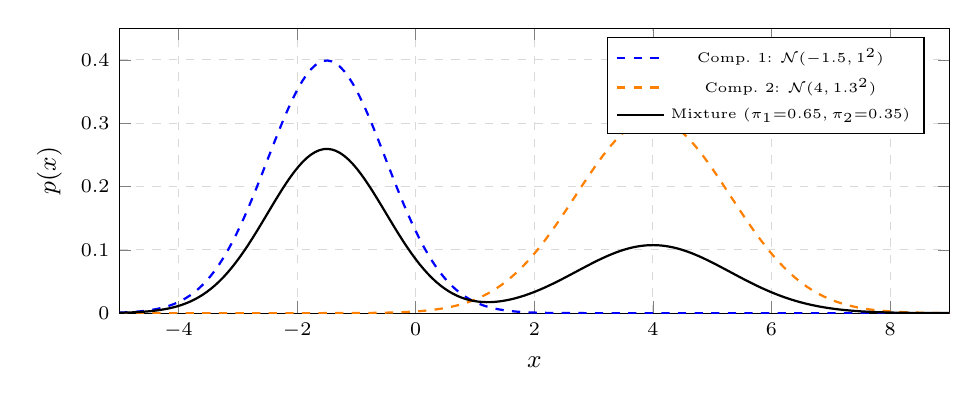
\begin{tikzpicture}
\begin{axis}[
    width=\linewidth, height=5.2cm,
    xlabel={$x$},
    ylabel={$p(x)$},
    xmin=-5, xmax=9,
    ymin=0, ymax=0.45,
    ytick={0, 0.1, 0.2, 0.3, 0.4},
    grid=major,
    grid style={dashed, gray!30},
    legend pos=north east,
    legend style={font=\tiny},
    tick label style={font=\scriptsize},
    label style={font=\small},
]
\addplot[blue, dashed, thick, domain=-5:9, samples=200]
    {1/sqrt(2*pi) * exp(-0.5*(x+1.5)^2)};
\addplot[orange, dashed, thick, domain=-5:9, samples=200]
    {1/sqrt(2*pi*1.69) * exp(-(x-4)^2/(2*1.69))};
\addplot[black, thick, domain=-5:9, samples=200]
    {0.65/sqrt(2*pi) * exp(-0.5*(x+1.5)^2)
     + 0.35/sqrt(2*pi*1.69) * exp(-(x-4)^2/(2*1.69))};
\addlegendentry{Comp.\ 1: $\mathcal{N}(-1.5,1^2)$}
\addlegendentry{Comp.\ 2: $\mathcal{N}(4,1.3^2)$}
\addlegendentry{Mixture ($\pi_1{=}0.65,\pi_2{=}0.35$)}
\end{axis}
\end{tikzpicture}
\caption{A two-component Gaussian Mixture Model. Each dashed curve is an individual component; the solid curve is their weighted sum. The mixture density is bimodal, whereas a single Gaussian would be forced to place mass between the two clusters.}
\label{fig:gmm_illustration}
\end{figure}

Because component assignment is a latent variable, GMM parameters are fitted by maximum likelihood using Expectation-Maximization (EM) \citep{dempster1977maximum}. The E-step computes the responsibility of component $m$ for observation $\mathbf{z}_i$,
\begin{equation}
    r_{im} = \frac{\pi_m \, \mathcal{N}(\mathbf{z}_i;\bm{\mu}_m,\bm{\sigma}_m^2)}{\sum_{m^\prime} \pi_{m^\prime}\,\mathcal{N}(\mathbf{z}_i;\bm{\mu}_{m^\prime},\bm{\sigma}_{m^\prime}^2)},
    \label{eq:resp}
\end{equation}
and the M-step updates parameters using effective counts $N_m=\sum_i r_{im}$:
\begin{align}
    \pi_m &= \frac{N_m}{N}, \qquad
    \bm{\mu}_m = \frac{1}{N_m}\sum_{i=1}^N r_{im}\mathbf{z}_i, \\
    \sigma_{mj}^2 &= \max\!\left(\frac{\sum_{i=1}^N r_{im}(z_{ij}-\mu_{mj})^2}{N_m},\sigma^2_{\min}\right),
    \label{eq:var_update}
\end{align}
where $\sigma^2_{\min}>0$ is a variance floor that prevents component collapse. Algorithm~\ref{alg:em_gmm} summarizes the procedure, alternating the E-step (Eq.~\eqref{eq:resp}) and the M-step (Eq.~\eqref{eq:var_update}) until the average log-likelihood converges.

\begin{algorithm}[t]
\caption{Expectation-Maximization for a Diagonal GMM}
\label{alg:em_gmm}
\KwIn{Observations $\{\mathbf{z}_i\}_{i=1}^N$; components $M$;\\ tolerance $\delta$; max steps $T_{\max}$}
\KwOut{Fitted $\{\pi_m, \bm{\mu}_m, \bm{\sigma}_m^2\}_{m=1}^M$}
Initialize $\pi_m \leftarrow 1/M$; sample $\bm{\mu}_m$ uniformly from $\{\mathbf{z}_i\}$; set $\bm{\sigma}_m^2$ to the global per-dimension variance\;
$\mathcal{L}^{(0)} \leftarrow -\infty$\;
\For{$t = 1, \ldots, T_{\max}$}{
    \textbf{E-step:} compute $r_{im}$ for all $i,m$ via Eq.~\eqref{eq:resp}\;
    \textbf{M-step:} update $\pi_m,\bm{\mu}_m,\bm{\sigma}_m^2$ for all $m$ via Eq.~\eqref{eq:var_update}\;
    $\mathcal{L}^{(t)} \leftarrow (1/N)\sum_{i=1}^N \log p(\mathbf{z}_i)$ via Eq.~\eqref{eq:logpk}\;
    \If{$|\mathcal{L}^{(t)} - \mathcal{L}^{(t-1)}| < \delta$}{\textbf{break}}
}
\Return $\{\pi_m, \bm{\mu}_m, \bm{\sigma}_m^2\}_{m=1}^M$\;
\end{algorithm}

GMM-based routing decides which adaptation module to apply to a given input by estimating how likely its feature representation is under each task's fitted density; this connects to the mixture-of-experts literature, in which a gating function assigns inputs to specialized expert networks \citep{jacobs1991adaptive,jordan1994hierarchical,shazeer2017outrageously,fedus2022switch}, reviewed further in Section~\ref{sec:related_work}. In the code domain, a single task often contains diverse subtypes --- algorithmic problems, string processing, data-structure manipulation --- that a single Gaussian cannot represent well; a mixture captures several sub-regions within the same task, and evaluating each task's fitted GMM on a frozen, task-agnostic representation provides a routing score without requiring task labels at inference time, motivating the routing mechanism developed in Section~\ref{sec:methodology}.

\section{Data Collection and Preprocessing}
\label{sec:data}

Two complementary benchmark tracks support the evaluation in this paper: a non-executable track scored by text-overlap metrics, and an executable track scored by unit-test execution. Figure~\ref{fig:pipeline_overview} summarizes the overall data pipeline, which proceeds through five stages: raw datasets are collected from multiple sources, schema-normalized to a common format, formatted using instruction templates, deduplicated to remove identical or near-identical examples, and partitioned into train, calibration, and test splits.

\begin{figure}[t]
\centering
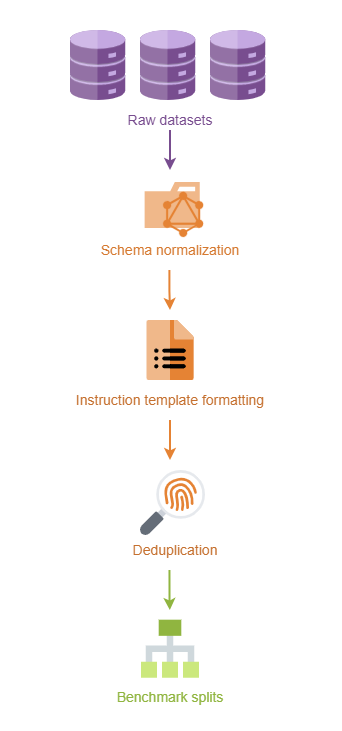
\includegraphics[width=\linewidth]{data_pipeline.png}
\caption{Data collection and preprocessing pipeline. Five sequential stages transform raw datasets from multiple diverse sources into clean, unified benchmark splits for both continual learning evaluation tracks.}
\label{fig:pipeline_overview}
\end{figure}

\subsection{The CodeTask benchmark}
\label{sec:codetask_data}

The CodeTask benchmark is the non-executable track used in this paper. It extends CodeTask-CL \citep{yadav2023exploring}, which combines generation, translation, summarization, and refinement tasks, with four additional tasks to create a longer and more diverse continual learning sequence. The original setting contains four tasks: English-to-Java generation using CONCODE \citep{iyer2018mapping}, Java-to-C\# translation using CodeXGLUE CodeTrans \citep{lu2021codexglue}, Ruby-to-English summarization using CodeSearchNet \citep{husain2019codesearchnet}, and Java-to-Java refinement using BFP \citep{tufano2019empirical}. We add Python generation using KodCode \citep{xu2025kodcode}, Ruby refinement using RunBugRun \citep{prenner2023runbugrun}, C\#-to-English summarization using the-vault-function \citep{nguyen2023vault}, and C++-to-C\# translation using CoST \citep{zhu2022multilingual}. Table~\ref{tab:codetask_stats} lists the eight tasks with their dataset sources and split sizes; Figure~\ref{fig:codetask_sequence} shows the resulting task order.

\begin{table}[t]
\centering
\caption{The CodeTask benchmark used in the non-executable continual learning track.}
\label{tab:codetask_stats}
\scriptsize
\resizebox{\linewidth}{!}{%
\begin{tabular}{llllrrr}
\toprule
Task & Dataset & In & Out & Train & Val. & Test \\
\midrule
Generation & CONCODE & English & Java & 100,000 & 2,000 & 2,000 \\
Translation & CodeXGLUE CodeTrans & Java & C\# & 10,300 & 500 & 1,000 \\
Summarization & CodeSearchNet & Ruby & English & 25,000 & 1,400 & 1,200 \\
Refinement & BFP & Java & Java & 46,600 & 5,800 & 5,800 \\
Generation & KodCode & English & Python & 100,000 & 5,000 & 5,000 \\
Refinement & RunBugRun & Ruby & Ruby & 10,000 & 972 & 1,000 \\
Summarization & the-vault-function & C\# & English & 100,000 & 5,000 & 5,000 \\
Translation & CoST & C++ & C\# & 12,000 & 272 & 410 \\
\bottomrule
\end{tabular}%
}
\end{table}

\begin{figure}[t]
\centering
\resizebox{\linewidth}{!}{%
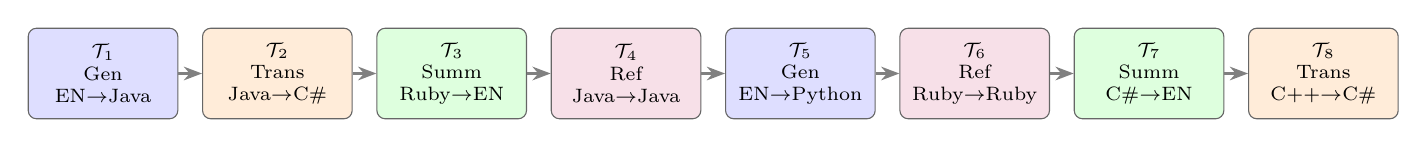
\begin{tikzpicture}[
  task/.style={rectangle, draw=black!60, rounded corners=3pt,
               minimum width=1.9cm, minimum height=1.15cm,
               text centered, align=center, font=\scriptsize, inner sep=3pt},
  gen/.style={task, fill=blue!13},
  trans/.style={task, fill=orange!15},
  summ/.style={task, fill=green!13},
  ref/.style={task, fill=purple!12},
  arr/.style={-Stealth, thick, draw=black!50}
]
\node[gen]   (t1) {$\mathcal{T}_1$\\Gen\\EN$\to$Java};
\node[trans, right=0.3cm of t1] (t2) {$\mathcal{T}_2$\\Trans\\Java$\to$C\#};
\node[summ,  right=0.3cm of t2] (t3) {$\mathcal{T}_3$\\Summ\\Ruby$\to$EN};
\node[ref,   right=0.3cm of t3] (t4) {$\mathcal{T}_4$\\Ref\\Java$\to$Java};
\node[gen,   right=0.3cm of t4] (t5) {$\mathcal{T}_5$\\Gen\\EN$\to$Python};
\node[ref,   right=0.3cm of t5] (t6) {$\mathcal{T}_6$\\Ref\\Ruby$\to$Ruby};
\node[summ,  right=0.3cm of t6] (t7) {$\mathcal{T}_7$\\Summ\\C\#$\to$EN};
\node[trans, right=0.3cm of t7] (t8) {$\mathcal{T}_8$\\Trans\\C++$\to$C\#};
\draw[arr](t1)--(t2); \draw[arr](t2)--(t3); \draw[arr](t3)--(t4);
\draw[arr](t4)--(t5); \draw[arr](t5)--(t6); \draw[arr](t6)--(t7);
\draw[arr](t7)--(t8);
\end{tikzpicture}}
\caption{The eight-task CodeTask continual learning sequence. Training data from earlier tasks are unavailable once the model advances past each task boundary. Node color indicates task type: blue for generation, orange for translation, green for summarization, purple for refinement.}
\label{fig:codetask_sequence}
\end{figure}

The additional tasks widen the range of languages and task types and introduce stronger distribution shifts: some tasks map natural language to code, some map code to code, and some map code to natural language. This mix makes the sequence more representative of real code-assistant workloads and better suited to studying when knowledge should transfer between tasks and when it should remain separated; restricting the sequence to one type of generation problem would risk conflating narrow adaptation with genuine continual learning ability.

Each dataset is cast into a unified instruction-style sequence-to-sequence format, since the source datasets use different schemas (natural-language intent and code snippet; buggy and repaired code; source code and docstring). To avoid the model relying on a single memorized prompt format, each example is wrapped with a template drawn from a pool of $N=20$ training templates per task type; at test time the pool expands to $M=30$ templates, so the test-time instructions include both familiar and unseen phrasing.

\subsection{The executable benchmark and deduplication pipeline}
\label{sec:exec_data}

The executable benchmark evaluates multilingual code generation under execution-based grading. Training data are drawn from OSS-Instruct \citep{wei2023magicoder} and McEval-Instruct \citep{chai2024mceval}; test data are drawn from McEval \citep{chai2024mceval}. All subsets cover the same nine programming languages: Python, C++, C\#, Java, Rust, Swift, PHP, TypeScript, and Shell. Unlike the CodeTask benchmark, each test example provides a problem description together with unit tests rather than a single reference output, and success is defined by whether the generated program passes the tests rather than by textual similarity to a reference solution, following the execution-based evaluation methodology of \citet{chen2021evaluating}.

Table~\ref{tab:exec_stats} summarizes the train, calibration, and test splits. OSS-Instruct is the largest training source (41,613 examples); McEval-Instruct adds 8,985 more balanced examples; McEval serves as the held-out test set. The calibration split --- used for candidate generation and for fitting the traceback router described in Section~\ref{sec:methodology} --- is assembled from the sanitized MBPP test split for Python \citep{austin2021program} and from the \texttt{mbpp-\textit{ext}} configuration of MultiPL-E for the remaining eight languages \citep{cassano2023multipl}; MultiPL-E does not provide reference solutions for these languages, so only pass/fail execution feedback is available for them. All calibration and test data are standardized to match the McEval instruction and test format.

\begin{table}[t]
\centering
\caption{Statistics of the executable benchmark subsets.}
\label{tab:exec_stats}
\scriptsize
\resizebox{\linewidth}{!}{%
\begin{tabular}{lrrrrrrrrrr}
\toprule
Split & Py & C++ & C\# & Java & Rust & Swift & PHP & TS & Shell & Total \\
\midrule
Train & 5,699 & 5,697 & 5,449 & 5,565 & 5,692 & 5,496 & 5,576 & 5,698 & 5,726 & 50,598 \\
Calib. & 426 & 397 & 386 & 386 & 354 & 396 & 397 & 390 & 382 & 3,514 \\
Test & 50 & 50 & 50 & 53 & 53 & 50 & 50 & 50 & 50 & 456 \\
\bottomrule
\end{tabular}%
}
\end{table}

The benchmark also brings multilingual adaptation into the continual learning setting: the same code-generation task repeats across nine languages that differ in syntax, standard libraries, and idiomatic patterns, so a continual learner may experience both positive transfer and interference across languages that the CodeTask benchmark, with its diversity of task types, does not directly test. Compared with CodeTask, the executable benchmark is narrower in task type but stronger in functional evaluation, isolating a single question: can the model keep learning to generate working programs across languages over time?

Because the executable benchmark is graded by execution, an undetected overlap between training and test examples would inflate reported scores by rewarding memorization rather than generalization, an effect that matters even more for a continual learner, whose apparent retention could otherwise reflect data leakage rather than genuine forward or backward transfer. The construction of the executable benchmark therefore includes a two-stage deduplication pipeline, illustrated in Figure~\ref{fig:near_dedup}.

\textbf{Exact deduplication.} Instruction text is whitespace-normalized and hashed with SHA-256 \citep{nist2015securehash}; examples sharing a hash are grouped into a cluster and reduced to one canonical representative. This stage removes verbatim copies but not near-identical problems that differ only by renamed identifiers or reworded descriptions.

\textbf{Near deduplication.} A stronger normalization is applied first --- Unicode normalization, prose/code separation, placeholder abstraction, identifier generalization to generic tokens, and import/punctuation normalization --- after which each example is represented as a set of token $n$-gram shingles. Comparing all shingle-set pairs directly is $O(N^2)$ and infeasible at scale, so MinHash is used to approximate Jaccard similarity efficiently: given $m$ independent hash functions, the signature of a shingle set $S$ is $\mathrm{MH}(S)=(\min_{s\in S}h_1(s),\ldots,\min_{s\in S}h_m(s))$, with the property $\Pr[\min h(S_A)=\min h(S_B)]=J(S_A,S_B)$ \citep{broder1997resemblance}. Locality-Sensitive Hashing (LSH) then restricts pairwise comparison to signatures sharing a band \citep{indyk1998approximate}, and each surviving candidate pair is scored with the exact Jaccard similarity $J(S_A,S_B)=|S_A\cap S_B|/|S_A\cup S_B|$ \citep{jaccard1901distribution}; a pair with $J\geq\theta$ is recorded as a near duplicate.

\begin{figure}[t]
\centering
\resizebox{\linewidth}{!}{%
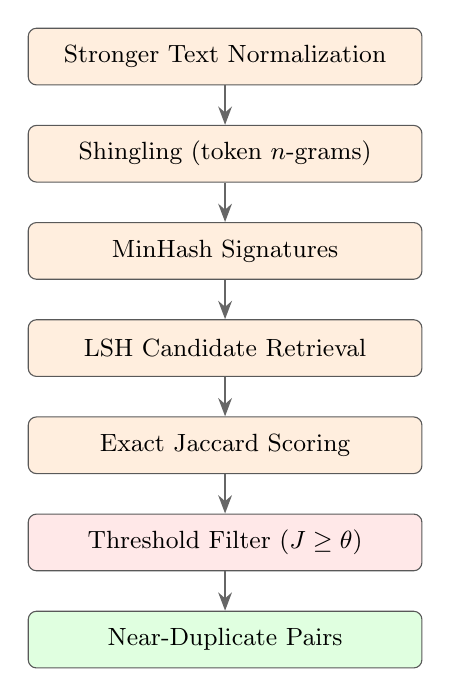
\begin{tikzpicture}[
  node distance=0.5cm,
  box/.style={rectangle, draw=black!65, rounded corners=3pt,
              minimum width=5.0cm, minimum height=0.72cm,
              text centered, font=\small, inner sep=4pt},
  procbox/.style={box, fill=orange!13},
  decbox/.style={box, fill=red!9},
  outbox/.style={box, fill=green!12},
  arr/.style={-Stealth, thick, draw=black!60},
]
\node[procbox] (norm) {Stronger Text Normalization};
\node[procbox, below=0.5cm of norm] (shin) {Shingling (token $n$-grams)};
\node[procbox, below=0.5cm of shin] (mh)   {MinHash Signatures};
\node[procbox, below=0.5cm of mh]   (lsh)  {LSH Candidate Retrieval};
\node[procbox, below=0.5cm of lsh]  (jac)  {Exact Jaccard Scoring};
\node[decbox,  below=0.5cm of jac]  (thr)  {Threshold Filter ($J \geq \theta$)};
\node[outbox,  below=0.5cm of thr]  (dup)  {Near-Duplicate Pairs};
\draw[arr](norm)--(shin); \draw[arr](shin)--(mh);
\draw[arr](mh)--(lsh);   \draw[arr](lsh)--(jac);
\draw[arr](jac)--(thr);  \draw[arr](thr)--(dup);
\end{tikzpicture}}
\caption{Near-deduplication pipeline. Normalization and shingling produce set representations; MinHash enables approximate similarity estimation; LSH restricts the search space to candidate pairs; exact Jaccard scoring provides the final decision.}
\label{fig:near_dedup}
\end{figure}

Exact-duplicate clusters are filtered and near-duplicate pairs that cross the train--test boundary are removed; this train--test filtering step is the primary safeguard against the model solving a test problem because it has seen an almost-identical version during training rather than because it generalized. The final stage standardizes all processed outputs into a common schema across splits, with shared fields index, language, instruction, solution, and test, so deduplication is integrated into the main benchmark construction pipeline rather than a separate post-hoc cleanup step.

\section{Methodology}
\label{sec:methodology}

This section presents GMM-Router, a framework for parameter-efficient continual code generation that routes each query to task-specific experts without retraining earlier adapters or retaining raw training data. GMM-Router has four components: task-specific LoRA expert training (Section~\ref{sec:experts}); routing feature extraction through a frozen backbone and a fixed orthonormal projection (Section~\ref{sec:features}); a continual GMM instruction router that supports hard and soft routing (Sections~\ref{sec:router} and~\ref{sec:soft_routing}); and, for the executable benchmark, an iterative refinement pipeline built around a second, traceback-based router (Section~\ref{sec:traceback}).

At a high level, GMM-Router processes the task sequence as follows. For each new task, a dedicated LoRA adapter and a GMM instruction router are trained in parallel (Sections~\ref{sec:experts}--\ref{sec:router}). At inference, the instruction router scores the query against every trained task and produces a routing distribution over adapters, which is used to select the highest-weighted adapter for hard routing or to merge all adapters for soft routing (Section~\ref{sec:soft_routing}); this constitutes Round-1 inference and is the only inference mechanism used on the CodeTask benchmark. On the executable benchmark, adapters are additionally evaluated on a held-out calibration split (Section~\ref{sec:setup}) whose failed predictions are used to refine each adapter on repair pairs and to fit a traceback GMM on error messages (Section~\ref{sec:traceback}); for any test sample whose five Round-1 candidates all fail execution, a second inference round combines the instruction and traceback routing signals through a Jensen--Shannon-divergence (JSD) gated rule to produce one additional prediction (Section~\ref{sec:round2}).

% ---------------------------------------------------------------------------
\subsection{Training task-specific experts}
\label{sec:experts}
% ---------------------------------------------------------------------------

For each task $\mathcal{T}_k$ with training dataset $\mathcal{D}_k$ (Eq.~\eqref{eq:dataset}), GMM-Router trains a task-specific LoRA adapter \citep{hu2022lora} on top of a shared frozen backbone, following the LoRA formulation in Section~\ref{sec:peft_background}. Each adapter is a low-rank update applied to the query and value projections in every transformer layer. Only the adapter parameters $\Theta_k=\{B_k^{(\ell)},A_k^{(\ell)}\}_\ell$ are updated; the backbone and all previously trained adapters remain frozen throughout training, so a new task cannot interfere with previously learned ones. The training objective is the negative log-likelihood of the target sequence,
\begin{equation}
    \mathcal{L}_k(\Theta_k) = -\sum_{(x,y)\in\mathcal{D}_k} \sum_{t=1}^{|y|}
    \log p_k(y_t \mid x, y_{<t}),
    \label{eq:task_loss}
\end{equation}
where $p_k(y_t\mid x,y_{<t})$ is the output distribution of expert $k$ at decoding step $t$. The backbone is split at layer $\ell^*$: layers $0$ through $\ell^*{-}1$ produce the frozen features used for routing (Section~\ref{sec:features}), while LoRA adapters modify layers $\ell^*$ through $L$. A larger $\ell^*$ dedicates more layers to routing features but leaves fewer layers for task-specific adaptation.

% ---------------------------------------------------------------------------
\subsection{Routing feature extraction}
\label{sec:features}
% ---------------------------------------------------------------------------

Stable routing requires a fixed representation space: if the feature map changed as new tasks arrived, GMMs fitted on earlier tasks would become misaligned with those fitted later. GMM-Router achieves this by extracting features from the frozen part of the backbone --- with all LoRA adapters disabled, so the routing space is independent of any per-task adapter weights --- and projecting them with a random matrix drawn once and fixed for the entire continual training run.

For a tokenized input of length $T$, the backbone produces hidden states $\mathbf{H}^{(\ell)}\in\mathbb{R}^{T\times d}$ at each layer $\ell$; the routing representation is taken at layer $\ell^*$, $\mathbf{H}=\mathbf{H}^{(\ell^*)}$. Using an intermediate layer yields representations that are less task-specific and more stable as tasks accumulate. The sequence-level representation is the mean of the token hidden states,
\begin{equation}
    \tilde{\mathbf{h}} = \frac{1}{T}\sum_{t=1}^{T} \mathbf{h}_t \in \mathbb{R}^d,
    \label{eq:meanpool}
\end{equation}
and parameter-free layer normalization removes scale differences,
\begin{equation}
    \mathbf{h} = \operatorname{LN}(\tilde{\mathbf{h}}), \qquad
    \operatorname{LN}(\mathbf{v}) = \frac{\mathbf{v} - \mu_{\mathbf{v}}}{\sigma_{\mathbf{v}} + \varepsilon},
    \label{eq:ln}
\end{equation}
where $\mu_\mathbf{v}$ and $\sigma_\mathbf{v}$ are the mean and standard deviation of the elements of $\mathbf{v}$. A fixed projection matrix $\mathbf{P}\in\mathbb{R}^{p\times d}$ then reduces the dimension to $p\ll d$: a random Gaussian matrix is drawn with a fixed seed, its thin QR factorization gives $\mathbf{P}$, so that $\mathbf{P}\mathbf{P}^\top=\mathbf{I}_p$. The routing embedding for input $x$ is
\begin{equation}
    \mathbf{z} = \mathbf{P}\,\mathbf{h} \in \mathbb{R}^p.
    \label{eq:z}
\end{equation}
Because $\mathbf{P}$ never changes, the routing embedding (Eq.~\eqref{eq:z}) lies in a fixed $p$-dimensional space for every task, so GMM densities fitted at any point in the sequence remain directly comparable to those fitted later.

% ---------------------------------------------------------------------------
\subsection{Continual GMM instruction router}
\label{sec:router}
% ---------------------------------------------------------------------------

Each task's instruction distribution is modeled as a diagonal GMM with $M$ components (Eq.~\eqref{eq:gmm}), fitted by EM (Algorithm~\ref{alg:em_gmm}) on the routing embeddings $\{\mathbf{z}_i^{(k)}\}_{i=1}^N$ of task $k$. When task $k$ arrives, its GMM is fitted and appended to the router registry; no parameters belonging to earlier tasks are modified.

\textbf{MAP scoring with a uniform class prior.} At inference, the router scores each registered task $k$ using the log-posterior under a uniform prior over the $K$ trained tasks,
\begin{equation}
    s_k(\mathbf{z}) = \log p_k(\mathbf{z}) + \log \frac{1}{K}.
    \label{eq:snorm}
\end{equation}
Since $\log(1/K)$ is constant across tasks, the argmax decision is equivalent to selecting the highest log-likelihood; the prior term keeps scores on a consistent scale as $K$ grows.

\textbf{Hard routing.} Given a query embedding $\mathbf{z}$, the hard router selects the task with the highest score,
\begin{equation}
    \hat{k} = \operatorname*{argmax}_{k \in \{1,\ldots,K\}} \; s_k(\mathbf{z}),
    \label{eq:routing}
\end{equation}
and generation proceeds using only expert $\hat{k}$'s adapter. This is the default inference strategy for the CodeTask benchmark.

% ---------------------------------------------------------------------------
\subsection{Soft routing and adapter merging}
\label{sec:soft_routing}
% ---------------------------------------------------------------------------

Rather than committing to a single expert, soft routing converts the log-posterior scores into a probability distribution over all $K$ tasks via a temperature-scaled softmax,
\begin{equation}
    \alpha_k(x) = \frac{\exp\!\left(s_k(\mathbf{z}) / \tau\right)}{\sum_{j=1}^K \exp\!\left(s_j(\mathbf{z}) / \tau\right)}, \qquad \bm{\alpha}(x) \in \Delta^{K-1},
    \label{eq:alpha}
\end{equation}
where $\tau>0$ is the routing temperature; as $\tau\to0^+$, $\bm{\alpha}(x)\to\mathbf{e}_{\hat{k}}$ recovers hard routing, and as $\tau\to\infty$, $\bm{\alpha}(x)\to\mathbf{1}/K$ becomes uniform. The $K$ LoRA adapters are then merged at the weight level,
\begin{equation}
    \Delta W_{\mathrm{merged}} = \sum_{k=1}^K \alpha_k(x)\, B_k A_k,
    \label{eq:weight_merge}
\end{equation}
yielding a single merged adapter applied to the frozen backbone for generation, at the cost of only one forward pass per decoding step regardless of $K$. Weight-level merging (Eq.~\eqref{eq:weight_merge}) approximates the mixture-of-experts output distribution $p_{\mathrm{mix}}(y_t\mid x,y_{<t})=\sum_k \alpha_k(x)\,p_k(y_t\mid x,y_{<t})$, which would otherwise require $K$ independent forward passes; because $\alpha_k(x)$ depends only on $x$, the routing weights are computed once per query and held fixed throughout autoregressive decoding. Algorithm~\ref{alg:generation} summarizes soft-routing generation, and Figure~\ref{fig:arch} illustrates the resulting Round-1 inference pipeline.

\begin{algorithm}[t]
\caption{Soft-Routing Expert-Mixture Generation}
\label{alg:generation}
\KwIn{Query $x$; log-posterior scores $\{s_k(\mathbf{z})\}$; adapters $\{(B_k, A_k)\}_{k=1}^K$; temperature $\tau$}
\KwOut{Generated output $\hat{y}$}
Extract routing embedding $\mathbf{z}$ with LoRA adapters disabled\;
$\alpha_k \leftarrow \exp(s_k(\mathbf{z})/\tau)/\sum_j\exp(s_j(\mathbf{z})/\tau)$, $\forall k$\;
Merge adapters: $\Delta W \leftarrow \sum_k \alpha_k B_k A_k$\;
Generate $\hat{y}$ with the merged adapter\;
\Return $\hat{y}$\;
\end{algorithm}

\begin{figure}[t]
\centering
\resizebox{\linewidth}{!}{%
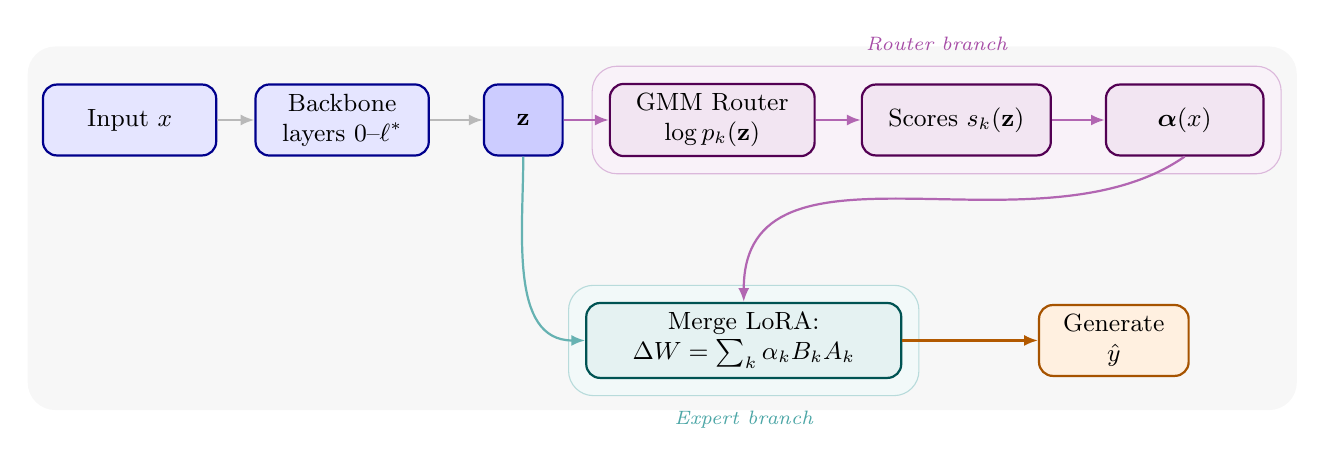
\begin{tikzpicture}[
    font=\small,
    shared/.style={draw=blue!55!black, line width=0.8pt, rounded corners=5pt,
        minimum width=2.2cm, minimum height=0.90cm, align=center, fill=blue!10},
    znode/.style={draw=blue!55!black, line width=0.8pt, rounded corners=5pt,
        minimum width=1.0cm, minimum height=0.90cm, align=center, fill=blue!20},
    rnode/.style={draw=violet!65!black, line width=0.8pt, rounded corners=5pt,
        minimum width=2.6cm, minimum height=0.90cm, align=center, fill=violet!10},
    enode/.style={draw=teal!65!black, line width=0.8pt, rounded corners=5pt,
        minimum width=1.9cm, minimum height=0.90cm, align=center, fill=teal!10},
    outnode/.style={draw=orange!65!black, line width=0.8pt, rounded corners=5pt,
        minimum width=1.9cm, minimum height=0.90cm, align=center, fill=orange!12},
    arr/.style= {-{Latex[length=5pt,width=4pt]}, thick, draw=gray!55},
    rarr/.style={-{Latex[length=5pt,width=4pt]}, thick, draw=violet!60},
    earr/.style={-{Latex[length=5pt,width=4pt]}, thick, draw=teal!60},
    oarr/.style={-{Latex[length=5pt,width=4pt]}, thick, draw=orange!70!black},
]
\node[shared]                          at ( 0.0, 0) (x)      {Input $x$};
\node[shared]                          at ( 2.7, 0) (enc)    {Backbone\\layers $0$--$\ell^*$};
\node[znode]                           at ( 5.0, 0) (z)      {$\mathbf{z}$};
\node[rnode]                           at ( 7.4, 0) (gmm)    {GMM Router\\$\log p_k(\mathbf{z})$};
\node[rnode, minimum width=2.4cm]      at (10.5, 0) (scores) {Scores $s_k(\mathbf{z})$};
\node[rnode, minimum width=2.0cm]      at (13.4, 0) (alpha)  {$\bm{\alpha}(x)$};
\draw[arr]  (x)      -- (enc);
\draw[arr]  (enc)    -- (z);
\draw[rarr] (z)      -- (gmm);
\draw[rarr] (gmm)    -- (scores);
\draw[rarr] (scores) -- (alpha);
\node[enode, minimum width=4.0cm] at (7.8, -2.8) (merge) {Merge LoRA:\\$\Delta W = \sum_k \alpha_k B_k A_k$};
\node[outnode] at (12.5, -2.8) (out) {Generate\\$\hat{y}$};
\draw[earr] (z.south) to[out=-90, in=180] (merge.west);
\draw[rarr] (alpha.south) to[out=-145, in=90] (merge.north);
\draw[oarr] (merge) -- (out);
\begin{scope}[on background layer]
    \fill[gray!6, rounded corners=10pt]
        ($(x.north west)+(-0.18, 0.47)$) rectangle ($(out.south east)+(1.36,-0.42)$);
    \node[draw=violet!28, fill=violet!5, rounded corners=9pt, inner sep=6pt,
          fit=(gmm)(scores)(alpha)] (rpanel) {};
    \node[draw=teal!28, fill=teal!5, rounded corners=9pt, inner sep=6pt,
          fit=(merge)] (epanel) {};
\end{scope}
\node[font=\scriptsize\itshape, violet!70] at (rpanel.north) [above=2pt] {Router branch};
\node[font=\scriptsize\itshape, teal!70]   at (epanel.south) [below=2pt] {Expert branch};
\end{tikzpicture}}
\caption{Round-1 inference pipeline of GMM-Router. The frozen backbone maps input $x$ to routing embedding $\mathbf{z}$ using layers $0$--$\ell^*$. The router branch (purple) evaluates the $K$ GMM log-densities, adds the uniform log-prior, and converts scores to routing weights $\bm{\alpha}(x)$. The expert branch (teal) merges the $K$ LoRA adapters as $\Delta W=\sum_k\alpha_k B_k A_k$ and generates output $\hat{y}$.}
\label{fig:arch}
\end{figure}

% ---------------------------------------------------------------------------
\subsection{Iterative refinement for executable code generation}
\label{sec:traceback}
% ---------------------------------------------------------------------------

For executable code generation, GMM-Router supports a second refinement round for samples where all Round-1 predictions fail execution. A separate GMM traceback router is trained on runtime error messages rather than instruction prompts, providing a complementary routing signal, and each per-task adapter is optionally refined on repair pairs; both procedures use the calibration predictions described in Section~\ref{sec:setup}.

\textbf{Traceback router.} The traceback router is a diagonal GMM (Section~\ref{sec:gmm_background}) fitted on error-message embeddings extracted from failed calibration predictions. For each failed candidate with a non-empty error string, the error text is collected and deduplicated; the resulting strings are encoded with the same frozen backbone used for instruction routing and projected into a separate routing space with its own fixed projection matrix, and a GMM is fitted per task using the EM procedure of Section~\ref{sec:gmm_background}.

\textbf{Adapter refinement.} In parallel with traceback router training, each per-task LoRA adapter can be further fine-tuned on repair pairs derived from the evaluated calibration data. Each pair consists of the original instruction, buggy code, and runtime traceback as input, paired with a ground-truth or passing candidate as target: for each calibration sample, the first failed candidate with a non-empty error string supplies the (buggy code, traceback) pair, and the repair target is the first passing candidate, or the ground-truth solution if none of the five candidates passed; samples with no failed candidate or no repair target are skipped.

\textbf{Round-2 inference and JSD-gated score combination.}
\label{sec:round2}
Round-2 inference applies only to samples where every Round-1 candidate failed. Let $\mathbf{s}_{\mathrm{in}}\in\mathbb{R}^K$ be the instruction router's Round-1 log-posterior scores and $\mathbf{s}_{\mathrm{tb}}\in\mathbb{R}^K$ the traceback router's scores on the corresponding error message; each is converted to a distribution, $\bm{\alpha}_{\mathrm{in}}=\operatorname{softmax}(\mathbf{s}_{\mathrm{in}}/\tau)$ and $\bm{\alpha}_{\mathrm{tb}}=\operatorname{softmax}(\mathbf{s}_{\mathrm{tb}})$. The two routers use fundamentally different signals --- natural-language problem descriptions versus runtime error messages --- so their agreement is informative about routing confidence: when both assign high probability to the same expert, that consensus is strong evidence the expert is correct; when they disagree, neither signal is fully trustworthy in isolation, and committing to either alone risks compounding the original routing error.

This motivates gating the combination by the degree of conflict between the two distributions. Let $\mathbf{m}=\tfrac{1}{2}(\bm{\alpha}_{\mathrm{in}}+\bm{\alpha}_{\mathrm{tb}})$. The Kullback--Leibler divergence from $p$ to $q$ is $\mathrm{KL}(p\|q)=\sum_k p_k\log(p_k/q_k)$ \citep{kullback1951information}, and the Jensen--Shannon divergence \citep{lin1991divergence} is its symmetrized, bounded variant,
\begin{equation}
    \mathrm{JSD}(\bm{\alpha}_{\mathrm{in}} \| \bm{\alpha}_{\mathrm{tb}})
    = \tfrac{1}{2}\mathrm{KL}(\bm{\alpha}_{\mathrm{in}}\|\mathbf{m})
    + \tfrac{1}{2}\mathrm{KL}(\bm{\alpha}_{\mathrm{tb}}\|\mathbf{m}).
    \label{eq:jsd}
\end{equation}
The combined routing weight is
\begin{equation}
    \bm{\alpha} = (1 - \mathrm{JSD})\operatorname{softmax}(\mathbf{s}_{\mathrm{in}} + \mathbf{s}_{\mathrm{tb}}) + \mathrm{JSD} \cdot \frac{\mathbf{1}}{K}.
    \label{eq:jsd_gated}
\end{equation}
When the two routers agree (low JSD), the combined log-posterior $\mathbf{s}_{\mathrm{in}}+\mathbf{s}_{\mathrm{tb}}$ is trusted and converted into a peaked distribution; when they disagree strongly (high JSD), the distribution is blended toward uniform, spreading probability mass across all experts rather than committing to a potentially wrong one. The rule in Eq.~\eqref{eq:jsd_gated} requires no additional learned parameters or tuned thresholds. The final Round-2 prediction is generated using $\bm{\alpha}$ and the same weight-level adapter merging as in Round-1 (Eq.~\eqref{eq:weight_merge}).

In summary, task-specific LoRA adapters prevent catastrophic forgetting through architectural isolation, since training on a new task updates only its dedicated adapter while all earlier adapters and the backbone remain frozen. Routing feature extraction projects frozen backbone representations through a fixed orthonormal matrix, keeping the routing space stable throughout the task sequence so GMM densities fitted at any point remain comparable as more tasks arrive. A per-task diagonal GMM fitted by EM models each task's instruction distribution and provides log-posterior scores for task-agnostic routing, realized as hard argmax selection for the CodeTask benchmark or temperature-scaled soft adapter merging for the executable benchmark; for the latter, the iterative refinement pipeline recovers samples that exhaust all Round-1 candidates by combining instruction and traceback routing signals through the JSD-gated rule.

\section{Evaluation}
\label{sec:evaluation}

\subsection{Research questions}
\label{sec:rqs}

The evaluation is organized around four research questions.

\noindent\textbf{RQ1.} How does GMM-Router perform relative to state-of-the-art continual learning baselines on a diverse, non-executable, eight-task code generation sequence?

\noindent\textbf{RQ2.} How does GMM-Router perform on a nine-language executable code generation benchmark judged by functional correctness, both on average and per programming language?

\noindent\textbf{RQ3.} To what extent does GMM-Router mitigate catastrophic forgetting and support knowledge transfer relative to the baselines, and how accurately does its GMM router assign inputs to the correct task-specific expert?

\noindent\textbf{RQ4.} Does the iterative refinement pipeline --- traceback routing combined with JSD-gated score combination --- improve performance on executable-benchmark samples that fail every Round-1 candidate?

\subsection{Datasets}
\label{sec:eval_datasets}

Both evaluation tracks introduced in Section~\ref{sec:data} are used: the eight-task CodeTask benchmark (Table~\ref{tab:codetask_stats}, Figure~\ref{fig:codetask_sequence}), scored with text-overlap metrics, addresses RQ1 and the routing-accuracy component of RQ3; the nine-language executable benchmark (Table~\ref{tab:exec_stats}), scored by unit-test execution, addresses RQ2 and RQ4, and its executable-track routing behavior additionally informs RQ3. Training proceeds through each benchmark's task sequence once, in the fixed order shown in Figure~\ref{fig:codetask_sequence} for CodeTask and the language order Python, C++, Swift, Rust, C\#, Java, PHP, TypeScript, Shell for the executable benchmark; validation after each task evaluates the model on every task seen so far, which is what makes the forgetting and transfer metrics defined in Section~\ref{sec:metrics} (Eqs.~\eqref{eq:fm}--\eqref{eq:bwt_fwt}) computable, while the tables in Section~\ref{sec:results} report the final scores after the full sequence has been learned. Maximum training size per task is capped at 100{,}000 examples, validation at 2{,}000, and test at 5{,}000, depending on the dataset (Table~\ref{tab:codetask_stats}).

\subsection{Configurations}
\label{sec:setup}

\subsubsection{Base model and baselines}
\label{sec:baselines}

All experiments use Qwen2.5-Coder-1.5B \citep{hui2024qwen25coder}, a decoder-only code language model (Section~\ref{sec:clm_background}) that is large enough to provide strong code-generation ability while remaining practical for repeated continual learning runs. GMM-Router is compared against seven continual learning baselines chosen to cover the main methodological directions (Section~\ref{sec:related_work}), plus one task-identity upper bound.

\emph{LoRA per task} trains an independent LoRA module per task with the backbone frozen and selects the module matching the true task label at inference \citep{hu2022lora}; because no adapter is ever overwritten, it removes catastrophic forgetting by construction and serves as an optimistic upper bound that requires task identity and storage that grows linearly with $K$. \emph{EWC} \citep{kirkpatrick2017overcoming} trains a single shared parameter set and penalizes changes to parameters the Fisher information marks as important for earlier tasks. \emph{L2P} \citep{wang2022learning} keeps the backbone frozen and learns a shared pool of soft prompts retrieved per input. \emph{ProgPrompt} \citep{razdaibiedina2023progressive} learns a new soft prompt per task while freezing previously learned prompts. \emph{SeqLoRA} trains one shared LoRA module sequentially across all tasks with no isolation mechanism, representing an aggressive, forgetting-prone form of parameter sharing. \emph{O-LoRA} \citep{wang2023orthogonal} extends sequential LoRA with an orthogonality constraint between successive task updates. \emph{Online-CL-LLM} \citep{cheng2025exploiting} characterizes each PEFT block by a representative feature distribution and dynamically selects blocks per input without task labels, making it the baseline methodologically closest to GMM-Router. \emph{TreeLoRA} \citep{qian2025treelora} organizes adapters in a hierarchical tree by gradient similarity between tasks, sharing structure between related tasks while separating unrelated ones. Table~\ref{tab:method_comparison} summarizes the baselines and GMM-Router along ten design properties.

\begin{table}[t]
\centering
\caption{Property comparison of baselines and GMM-Router. \ymark{} = has property; \xmark{} = lacks property. \textbf{Back.} = backbone frozen; \textbf{Isol.} = dedicated module per task; \textbf{Agn.} = no task identity needed at inference; \textbf{Repl.} = stores/replays raw data; \textbf{Rout.} = routes via learned feature distributions; \textbf{Shar.} = models cross-task parameter relationships; \textbf{Reg.} = applies parameter regularization; \textbf{Refine.} = iteratively refines failed predictions using execution feedback.}
\label{tab:method_comparison}
\scriptsize
\resizebox{\linewidth}{!}{%
\begin{tabular}{lcccccccccc}
\toprule
Method & Back. & Isol. & Agn. & Repl. & LoRA & Prompt & Rout. & Shar. & Reg. & Refine. \\
\midrule
LoRA per task  & \ymark & \ymark & \xmark & \xmark & \ymark & \xmark & \xmark & \xmark & \xmark & \xmark \\
EWC            & \xmark & \xmark & \ymark & \xmark & \xmark & \xmark & \xmark & \xmark & \ymark & \xmark \\
L2P            & \ymark & \xmark & \ymark & \xmark & \xmark & \ymark & \xmark & \xmark & \xmark & \xmark \\
ProgPrompt     & \ymark & \ymark & \ymark & \xmark & \xmark & \ymark & \xmark & \xmark & \xmark & \xmark \\
SeqLoRA        & \ymark & \xmark & \ymark & \xmark & \ymark & \xmark & \xmark & \xmark & \xmark & \xmark \\
O-LoRA         & \ymark & \xmark & \ymark & \xmark & \ymark & \xmark & \xmark & \xmark & \ymark & \xmark \\
Online-CL-LLM  & \ymark & \ymark & \ymark & \xmark & \ymark & \xmark & \ymark & \xmark & \xmark & \xmark \\
TreeLoRA       & \ymark & \xmark & \ymark & \xmark & \ymark & \xmark & \xmark & \ymark & \xmark & \xmark \\
\midrule
\textbf{GMM-Router} & \ymark & \ymark & \ymark & \xmark & \ymark & \xmark & \ymark & \xmark & \xmark & \ymark \\
\bottomrule
\end{tabular}%
}
\end{table}

\subsubsection{Hyperparameters}
\label{sec:hyperparams}

For the CodeTask benchmark, the eight-task order follows Figure~\ref{fig:codetask_sequence}; for the executable benchmark, the nine-language order is Python, C++, Swift, Rust, C\#, Java, PHP, TypeScript, Shell. All methods train for 3 epochs per task with batch size 32, learning rate $10^{-4}$, warmup ratio 0.01, and weight decay 0.01. Padding tokens are masked in the labels (target value $-100$) so they do not contribute to the loss, and long inputs are truncated based on each dataset's input-length distribution.

LoRA-based methods use rank $r=16$, $\mathtt{lora\_alpha}=32$, $\mathtt{lora\_dropout}=0.1$, applied to the attention query and value projections (\texttt{q\_proj}, \texttt{v\_proj}) with no trained bias parameters. After each adapter is trained, it is run on the held-out calibration split to generate $n=5$ candidate predictions per problem (temperature $0.2$, top-$p=0.95$); the stored output --- instruction, five candidates, pass/fail result, and error string per failed candidate --- feeds both the traceback router and adapter refinement. Table~\ref{tab:router_comparison} compares the instruction and traceback router hyperparameters; the traceback router's higher EM iteration budget compensates for its smaller, post-deduplication training set, and its input is truncated from the left so the final lines of a traceback --- which carry the error type and message --- are preserved. Adapter refinement continues training the existing per-task adapter at learning rate $5\times10^{-5}$ for 3 epochs, weight decay $0.01$, effective batch size 8, and a maximum prompt length of 4096 tokens to accommodate the concatenated instruction, buggy code, and traceback.

\begin{table}[t]
\centering
\caption{Hyperparameters of the instruction and traceback routers.}
\label{tab:router_comparison}
\small
\begin{tabular}{lcc}
\toprule
Hyperparameter & Instruction & Traceback \\
\midrule
Routing layer $\ell^*$ & 4 & 4 \\
Routing dimension $p$ & 256 & 256 \\
Max input length & 2048 & 256 \\
Truncation side & right & left \\
Variance floor $\sigma^2_{\min}$ & 0.02 & $10^{-3}$ \\
EM max iterations $T_{\max}$ & 50 & 100 \\
EM tolerance $\delta$ & $10^{-4}$ & $10^{-4}$ \\
GMM components $M$ & 4 & 4 \\
Training samples & up to 5{,}000 & up to 600 \\
\bottomrule
\end{tabular}
\end{table}

For Round-1 inference, the routing temperature is $\tau=1.0$. On the CodeTask benchmark, hard routing is used with generation temperature $0.2$, top-$p=0.95$, and up to 512 newly generated tokens. On the executable benchmark, soft routing is used, generating 5 candidates per sample (up to 2048 tokens) to support Pass@$k$ evaluation. Round-2 inference applies only to the executable benchmark: per-router temperatures default to $1.0$ and failed samples produce one new prediction with greedy decoding.

\subsubsection{Evaluation metrics}
\label{sec:metrics}

The non-executable and executable tracks use different metrics because they capture different aspects of code generation quality. For the non-executable benchmark, BLEU \citep{papineni2002bleu} measures $n$-gram overlap between a generated sequence and one or more references using modified precision $p_n$ (each $n$-gram count in the hypothesis clipped by its maximum occurrence across references) and a brevity penalty $\mathrm{BP}$ that equals 1 when the hypothesis is at least as long as the reference and $\exp(1-r/c)$ otherwise, for hypothesis length $c$ and reference length $r$:
\begin{equation}
\mathrm{BLEU} = \mathrm{BP} \cdot \exp\!\left(\sum_{n=1}^{4} \tfrac{1}{4} \log p_n\right).
\label{eq:bleu}
\end{equation}
CodeBLEU \citep{ren2020codebleu} extends BLEU with code-specific components, since code quality depends on syntactic and semantic structure as well as token overlap:
\begin{align}
\mathrm{CodeBLEU} ={} & \alpha \cdot \mathrm{NgramMatch} \notag \\
& + \beta \cdot \mathrm{WeightedNgramMatch} \notag \\
& + \gamma \cdot \mathrm{SyntaxMatch} \notag \\
& + \delta \cdot \mathrm{DataflowMatch},
\label{eq:codebleu}
\end{align}
with $\alpha=\beta=\gamma=\delta=0.25$. \texttt{NgramMatch} is standard BLEU-style precision; \texttt{WeightedNgramMatch} up-weights language keywords and operators; \texttt{SyntaxMatch} compares abstract syntax trees by tree-edit distance; \texttt{DataflowMatch} compares variable-level data-flow relations, capturing semantic equivalence that token matching misses. Neither metric can fully distinguish code that is functionally correct from code that merely looks similar to a reference, which motivates the executable track.

For the executable benchmark, the main metric is Pass@$k$ \citep{chen2021evaluating}: the probability that at least one of $k\leq n$ sampled candidates passes all unit tests, given $n$ sampled candidates of which $c$ pass,
\begin{equation}
\mathrm{Pass@}k = 1 - \frac{\binom{n-c}{k}}{\binom{n}{k}},
\label{eq:passk}
\end{equation}
defined as $1$ when $n-c<k$. This paper reports Pass@1 (whether the first candidate is correct) and Pass@5 (whether any of five candidates is correct), which is informative in multilingual code generation where a problem may admit several correct implementations. Together, BLEU, CodeBLEU, and Pass@$k$ let this paper evaluate both textual quality and functional correctness across the two complementary benchmark settings.

Three further metrics quantify continual learning behavior on top of either per-task metric: BLEU/CodeBLEU on the CodeTask benchmark, or Pass@$k$ on the executable benchmark. Let $a_{i,j}$ denote the per-task metric value on task $\mathcal{T}_j$ after training on tasks $\mathcal{T}_1,\ldots,\mathcal{T}_i$. The Forgetting Measure (FM) \citep{wang2023comprehensive} captures the drop from each task's best observed performance to its current performance:
\begin{equation}
f_{j,k} = \max_{i \in \{1,\ldots,k-1\}} (a_{i,j} - a_{k,j}), \qquad
\mathrm{FM}_k = \frac{1}{k-1}\sum_{j=1}^{k-1} f_{j,k}.
\label{eq:fm}
\end{equation}
Backward Transfer (BWT) measures how training on later tasks affects earlier ones:
\begin{equation}
\mathrm{BWT}_k = \frac{1}{k-1}\sum_{j=1}^{k-1}(a_{k,j}-a_{j,j}).
\label{eq:bwt}
\end{equation}
Forward Transfer (FWT) measures the extent to which learning previous tasks improves the model's performance on a new task before the model is trained on that task:
\begin{equation}
\mathrm{FWT}_k = \frac{1}{k-1}\sum_{j=2}^{k}\left(a_{j-1,j} - a_{0,j}\right),
\label{eq:bwt_fwt}
\end{equation}
where $a_{j-1,j}$ is the performance on task $\mathcal{T}_j$ after training on tasks $\mathcal{T}_1,\ldots,\mathcal{T}_{j-1}$ but before training on $\mathcal{T}_j$, and $a_{0,j}$ is the performance of the initial pretrained model on task $\mathcal{T}_j$ prior to any continual-learning training; $a_{j-1,j}-a_{0,j}$ thus quantifies the change in zero-shot performance on task $\mathcal{T}_j$ resulting from learning the preceding tasks. This definition follows the forward-transfer metric introduced by \citet{lopezpaz2017gem}, with the randomly initialized reference performance replaced by the initial pretrained-model performance, which provides a more meaningful baseline for pretrained code language models. Negative BWT indicates net forgetting; a positive FWT value indicates that knowledge acquired from previous tasks improves generalization to unseen tasks, a negative value indicates that previous training reduces the model's initial ability to perform the new task, and a value close to zero indicates that learning the preceding tasks has little effect on performance on future tasks.

\section{Experimental Results}
\label{sec:results}

This section reports and discusses results for the four research questions in Section~\ref{sec:rqs}. LoRA per task serves as the upper-bound reference in every comparison because it uses the true task label at inference; every other method, including GMM-Router, must infer the task from the input alone.

\subsection{RQ1: Performance on the CodeTask benchmark}
\label{sec:codetask_results}

Table~\ref{tab:codetask_qwen} reports the final per-task and average scores on the CodeTask benchmark after the model has learned the full eight-task sequence.

\begin{table}[t]
\centering
\caption{Final results (\%) on the CodeTask benchmark (Qwen2.5-Coder-1.5B, $\tau=2.0$). LoRA per task is the upper bound (task identity known at inference).}
\label{tab:codetask_qwen}
\scriptsize
\resizebox{\linewidth}{!}{%
\begin{tabular}{lccccccccc}
\toprule
Method & CONCODE & CodeTrans & CodeSearchNet & BFP & KodCode & RunBugRun & TheVault & CoST & Avg. \\
\midrule
LoRA per task & 36.56 & 77.55 & 16.00 & 80.15 & 54.20 & 66.11 & 26.48 & 76.17 & 54.15 \\
\midrule
EWC & 8.54 & 17.79 & 2.73 & 41.48 & 8.74 & 37.56 & 18.28 & 70.40 & 25.69 \\
L2P & 5.62 & 23.32 & 2.60 & 35.09 & 6.36 & 24.98 & 2.21 & 34.34 & 16.82 \\
ProgPrompt & 11.83 & 34.34 & 1.88 & 35.90 & 15.93 & 18.23 & 1.87 & 68.90 & 23.61 \\
SeqLoRA & 14.04 & 37.96 & 1.99 & 62.64 & 20.02 & 64.10 & 2.53 & 75.92 & 34.90 \\
O-LoRA & 10.84 & 36.09 & 13.80 & 77.24 & 41.77 & 65.89 & 21.21 & 75.34 & 42.77 \\
Online-CL-LLM & 22.52 & 47.97 & 14.65 & 68.57 & 25.22 & 64.83 & 15.24 & 71.87 & 41.36 \\
TreeLoRA & 14.85 & 34.58 & 2.12 & 44.24 & 17.27 & 78.18 & 2.16 & 83.20 & 34.58 \\
\midrule
\textbf{GMM-Router} & 35.06 & 73.48 & 14.85 & 79.95 & 51.75 & 63.12 & 18.51 & 76.26 & 51.62 \\
\bottomrule
\end{tabular}%
}
\end{table}

GMM-Router reaches the highest average (51.62\%) among all task-agnostic methods, ahead of O-LoRA (42.77\%) and Online-CL-LLM (41.36\%) by a wide margin and close to the LoRA per task upper bound (54.15\%). The advantage stems from three design choices acting together (Section~\ref{sec:methodology}): task-isolated LoRA adapters that prevent gradient interference, a stable routing space from the fixed orthonormal projection $\mathbf{P}$ applied to frozen backbone features, and hard routing that assigns each input deterministically to its best-matching expert via GMM log-posteriors under a uniform class prior.

GMM-Router is strongest on BFP (79.95\%), CoST (76.26\%), and CodeTrans (73.48\%), all close to or matching the upper bound, indicating that dedicated experts with stable routing suffice for these structured tasks. It is weaker on TheVault (18.51\%) and CodeSearchNet (14.85\%), both code-to-text generation tasks whose broad, less distinctive input distributions are harder to separate by density estimation alone. Among the baselines, O-LoRA and Online-CL-LLM are strongest, reflecting the benefit of orthogonal subspaces and feature-based block selection, respectively; SeqLoRA (34.90\%) and TreeLoRA (34.58\%) trail, and EWC (25.69\%), ProgPrompt (23.61\%), and L2P (16.82\%) are substantially weaker, indicating that shallow regularization or limited prompt capacity is insufficient for this diverse benchmark.

\subsection{RQ2: Performance on the executable benchmark}
\label{sec:exec_results}

Table~\ref{tab:exec_avg} reports average Pass@1 and Pass@5 on the executable benchmark.

\begin{table}[t]
\centering
\caption{Average Pass@1 and Pass@5 (\%) on the executable benchmark. LoRA per task is the upper bound (task identity known, without iterative refinement).}
\label{tab:exec_avg}
\small
\begin{tabular}{lcc}
\toprule
Method & Avg.\ Pass@1 (\%) & Avg.\ Pass@5 (\%) \\
\midrule
LoRA per task & 33.46 & 42.19 \\
\midrule
EWC & 0.09 & 0.22 \\
L2P & 8.03 & 11.75 \\
ProgPrompt & 28.01 & 40.00 \\
SeqLoRA & 37.51 & 45.67 \\
O-LoRA & 33.71 & 42.09 \\
Online-CL-LLM & 33.50 & 41.95 \\
TreeLoRA & 36.84 & 46.37 \\
\midrule
\textbf{GMM-Router} & 34.40 & 47.75 \\
\bottomrule
\end{tabular}
\end{table}

GMM-Router reaches 34.40\% Pass@1 and 47.75\% Pass@5. On Pass@1, SeqLoRA (37.51\%) and TreeLoRA (36.84\%) lead, benefiting from cross-task transfer that a shared or hierarchically shared adaptation space provides on this benchmark, which is homogeneous in task format across nine syntactically related languages. On Pass@5, GMM-Router leads all methods (47.75\%), ahead of TreeLoRA (46.37\%) and SeqLoRA (45.67\%), indicating that soft routing produces a more diverse candidate set that collectively covers more of the problem space. GMM-Router's Pass@1 (34.40\%) slightly exceeds the non-iterative LoRA per task upper bound (33.46\%); this improvement is attributable to the iterative refinement pipeline recovering samples that fail every Round-1 candidate (RQ4, Section~\ref{sec:refinement}). GMM-Router also outperforms O-LoRA (33.71\%/42.09\%) and Online-CL-LLM (33.50\%/41.95\%), consistent with per-task GMM density estimation in a stable, fixed-projection routing space providing a more reliable task-distribution model than orthogonality constraints or feature-distribution matching alone. EWC (0.09\% Pass@1) and L2P (8.03\%) perform poorly, indicating that regularization and shallow prompt selection are insufficient for generating functionally correct multilingual code. The gap to SeqLoRA ($-3.11$pp Pass@1) reflects a trade-off examined further in Section~\ref{sec:crossbench}: SeqLoRA's shared adaptation accumulates cross-language knowledge on this homogeneous benchmark but forgets severely on the diverse CodeTask sequence (34.90\% vs.\ GMM-Router's 51.62\%, Table~\ref{tab:codetask_qwen}).

\subsubsection{Per-language analysis}
\label{sec:perlang}

Tables~\ref{tab:exec_p1} and~\ref{tab:exec_p5} report Pass@1 and Pass@5 for each programming language.

\begin{table}[t]
\centering
\caption{Per-language Pass@1 (\%) on the executable benchmark ($\tau=1.0$).}
\label{tab:exec_p1}
\scriptsize
\resizebox{\linewidth}{!}{%
\begin{tabular}{lccccccccc}
\toprule
Method & Py & C++ & Swift & Rust & C\# & Java & PHP & TS & Shell \\
\midrule
LoRA per task & 43.59 & 6.80 & 59.20 & 22.64 & 1.20 & 18.87 & 36.40 & 93.20 & 19.20 \\
\midrule
EWC & 0.80 & 0.00 & 0.00 & 0.00 & 0.00 & 0.00 & 0.00 & 0.00 & 0.00 \\
L2P & 7.60 & 2.40 & 24.80 & 1.51 & 7.60 & 0.00 & 10.80 & 17.60 & 0.00 \\
ProgPrompt & 31.60 & 16.80 & 57.20 & 4.15 & 3.60 & 13.96 & 30.80 & 78.80 & 15.20 \\
SeqLoRA & 45.52 & 13.60 & 62.00 & 10.57 & 24.00 & 22.26 & 33.20 & 98.40 & 28.00 \\
O-LoRA & 42.40 & 11.20 & 63.60 & 11.70 & 0.80 & 18.49 & 36.80 & 95.20 & 23.20 \\
Online-CL-LLM & 42.80 & 21.20 & 42.00 & 8.30 & 25.20 & 20.75 & 30.80 & 90.80 & 19.60 \\
TreeLoRA & 42.80 & 4.40 & 63.60 & 32.08 & 14.80 & 21.51 & 34.40 & 95.60 & 22.40 \\
\midrule
\textbf{GMM-Router} & 38.40 & 5.60 & 66.40 & 19.62 & 2.80 & 23.40 & 34.80 & 92.80 & 25.80 \\
\bottomrule
\end{tabular}%
}
\end{table}

\begin{table}[t]
\centering
\caption{Per-language Pass@5 (\%) on the executable benchmark ($\tau=1.0$).}
\label{tab:exec_p5}
\scriptsize
\resizebox{\linewidth}{!}{%
\begin{tabular}{lccccccccc}
\toprule
Method & Py & C++ & Swift & Rust & C\# & Java & PHP & TS & Shell \\
\midrule
LoRA per task & 54.00 & 8.00 & 72.00 & 35.85 & 4.00 & 35.85 & 44.00 & 96.00 & 30.00 \\
\midrule
EWC & 2.00 & 0.00 & 0.00 & 0.00 & 0.00 & 0.00 & 0.00 & 0.00 & 0.00 \\
L2P & 14.00 & 4.00 & 30.00 & 3.77 & 14.00 & 0.00 & 14.00 & 26.00 & 0.00 \\
ProgPrompt & 46.00 & 32.00 & 76.00 & 9.43 & 8.00 & 24.53 & 48.00 & 92.00 & 24.00 \\
SeqLoRA & 54.00 & 18.00 & 74.00 & 20.75 & 36.00 & 28.30 & 38.00 & 100.00 & 42.00 \\
O-LoRA & 56.00 & 14.00 & 72.00 & 24.53 & 4.00 & 28.30 & 46.00 & 100.00 & 34.00 \\
Online-CL-LLM & 50.00 & 30.00 & 54.00 & 11.32 & 32.00 & 30.19 & 40.00 & 98.00 & 32.00 \\
TreeLoRA & 54.00 & 8.00 & 70.00 & 50.94 & 24.00 & 26.42 & 44.00 & 100.00 & 40.00 \\
\midrule
\textbf{GMM-Router} & 46.00 & 8.00 & 80.00 & 58.49 & 8.00 & 45.28 & 46.00 & 100.00 & 38.00 \\
\bottomrule
\end{tabular}%
}
\end{table}

GMM-Router leads all methods on Swift (66.40\% Pass@1, 80.00\% Pass@5) and on Java Pass@5 (45.28\%, well above the next best, SeqLoRA and O-LoRA at 28.30\%), suggesting soft routing produces diverse candidates that cover more of the Java problem space. TypeScript is the easiest language overall (92.80\% Pass@1, 100.00\% Pass@5 for GMM-Router and most strong baselines). Rust shows a diversity benefit from soft routing: GMM-Router's Pass@1 (19.62\%) trails TreeLoRA (32.08\%), yet its Pass@5 (58.49\%) exceeds TreeLoRA's (50.94\%). GMM-Router is weakest on C\# (2.80\%/8.00\%) and C++ (5.60\%/8.00\%); for C\#, methods with shared adaptation (SeqLoRA 24.00\%, Online-CL-LLM 25.20\%) perform substantially better, suggesting C\# benefits from cross-language transfer that per-task isolation cannot exploit. Python (38.40\% Pass@1) similarly falls behind SeqLoRA (45.52\%), consistent with a Python distribution close enough to other languages in this benchmark that shared adaptation provides a useful inductive bias.

\subsection{RQ3: Forgetting, transfer, and router assignment}
\label{sec:rq3}

\subsubsection{Router assignment analysis}
\label{sec:routing_analysis}

To understand which task distributions the GMM router can reliably separate, this subsection examines hard-routing confusion matrices ($\hat k=\operatorname{argmax}_k\alpha_k(x)$) at the final training step. On CodeTask, hard routing is the actual inference method; on the executable benchmark, Round-1 uses soft routing, so this analysis instead exposes where the argmax decision fails and motivates the traceback router used in Round-2.

\paragraph{CodeTask benchmark.} Figure~\ref{fig:confusion_codetask} shows the row-normalized confusion matrix after the full eight-task sequence (percentage of 1{,}000 test samples per true task hard-routed to each expert). The average accuracy is 90.6\%. BFP (98.3\%) and CoST (99.5\%) are routed almost perfectly because their distinctive input/output language combinations (Java bug patches; C++ source with C\# target) produce compact, well-separated GMM regions. The two weakest tasks are TheVault (82.6\%) and RunBugRun (86.4\%). Two systematic confusion patterns explain most off-diagonal mass: CodeTrans draws 10.8\% of TheVault and 5.8\% of CONCODE samples because all three tasks share Java or C\# as an input or output language; and CoST draws 9.0\% of RunBugRun, 8.6\% of CodeTrans, 6.7\% of KodCode, and 6.6\% of TheVault, reflecting both its C\# output overlapping with CodeTrans/TheVault and code-to-code transformation tasks sharing structural embedding patterns with translation. These confusions align with the performance gaps in Table~\ref{tab:codetask_qwen}: TheVault and RunBugRun show the largest gaps to their per-task upper bounds.

\begin{figure}[t]
\centering
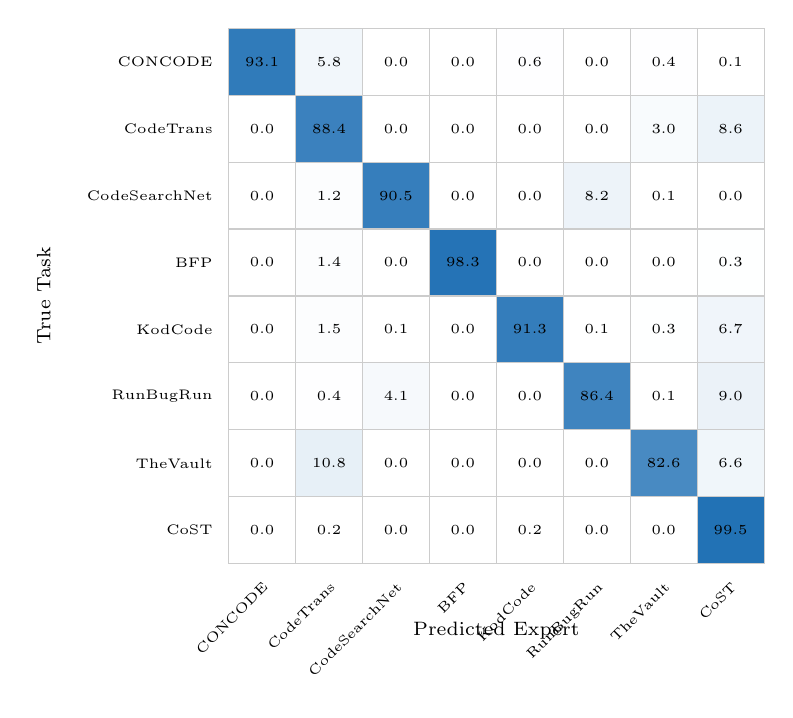
\begin{tikzpicture}
  \foreach \r/\c/\v in {
    0/0/93.1, 0/1/5.8,  0/2/0.0,  0/3/0.0,  0/4/0.6,  0/5/0.0,  0/6/0.4,  0/7/0.1,
    1/0/0.0,  1/1/88.4, 1/2/0.0,  1/3/0.0,  1/4/0.0,  1/5/0.0,  1/6/3.0,  1/7/8.6,
    2/0/0.0,  2/1/1.2,  2/2/90.5, 2/3/0.0,  2/4/0.0,  2/5/8.2,  2/6/0.1,  2/7/0.0,
    3/0/0.0,  3/1/1.4,  3/2/0.0,  3/3/98.3, 3/4/0.0,  3/5/0.0,  3/6/0.0,  3/7/0.3,
    4/0/0.0,  4/1/1.5,  4/2/0.1,  4/3/0.0,  4/4/91.3, 4/5/0.1,  4/6/0.3,  4/7/6.7,
    5/0/0.0,  5/1/0.4,  5/2/4.1,  5/3/0.0,  5/4/0.0,  5/5/86.4, 5/6/0.1,  5/7/9.0,
    6/0/0.0,  6/1/10.8, 6/2/0.0,  6/3/0.0,  6/4/0.0,  6/5/0.0,  6/6/82.6, 6/7/6.6,
    7/0/0.0,  7/1/0.2,  7/2/0.0,  7/3/0.0,  7/4/0.2,  7/5/0.0,  7/6/0.0,  7/7/99.5%
  } {
    \fill[heatblue!\v!white]
      ({\c*\CTcs}, {-\r*\CTcs}) rectangle ({(\c+1)*\CTcs}, {-(\r+1)*\CTcs});
    \node[font=\tiny] at ({(\c+0.5)*\CTcs}, {-(\r+0.5)*\CTcs}) {\v};
  }
  \draw[gray!40, thin] (0,0) grid[xstep=\CTcs, ystep=\CTcs] ({8*\CTcs},{-8*\CTcs});
  \foreach \c/\lbl in {
    0/CONCODE, 1/CodeTrans, 2/CodeSearchNet, 3/BFP,
    4/KodCode, 5/RunBugRun, 6/TheVault, 7/CoST%
  } {
    \node[font=\tiny, anchor=north east, rotate=45]
      at ({(\c+0.5)*\CTcs}, {-8*\CTcs-0.05}) {\lbl};
  }
  \foreach \r/\lbl in {
    0/CONCODE, 1/CodeTrans, 2/CodeSearchNet, 3/BFP,
    4/KodCode, 5/RunBugRun, 6/TheVault, 7/CoST%
  } {
    \node[font=\tiny, anchor=east]
      at ({-0.08}, {-(\r+0.5)*\CTcs}) {\lbl};
  }
  \node[font=\scriptsize] at ({4*\CTcs}, {-9.0*\CTcs}) {Predicted Expert};
  \node[font=\scriptsize, rotate=90, anchor=center] at (-2.35, {-4*\CTcs}) {True Task};
\end{tikzpicture}
\caption{Hard-routing confusion matrix (\%) on the CodeTask benchmark at the final training step. Rows = true task; columns = assigned expert. Diagonal entries indicate correct routing; darker cells indicate higher routing weight.}
\label{fig:confusion_codetask}
\end{figure}

\paragraph{Executable benchmark.} Figure~\ref{fig:confusion_exec} shows the instruction router's confusion matrix after the full nine-language sequence. The average accuracy is only 15.8\%, sharply lower than on CodeTask. C++ dominates as a single attractor, drawing between 60\% (Python) and 100\% (C++ itself and TypeScript) of every language's samples; Python is the only exception, correctly routing 40.0\% of its own samples, while all other non-C++ languages score at most 2.0\%. This collapse occurs because the nine languages share deep syntactic overlap --- C-style braces, type keywords, similar control-flow constructs --- and because C++, trained second in the sequence, established broad coverage of the routing feature space before later languages' GMMs could carve out well-separated regions.

\begin{figure}[t]
\centering
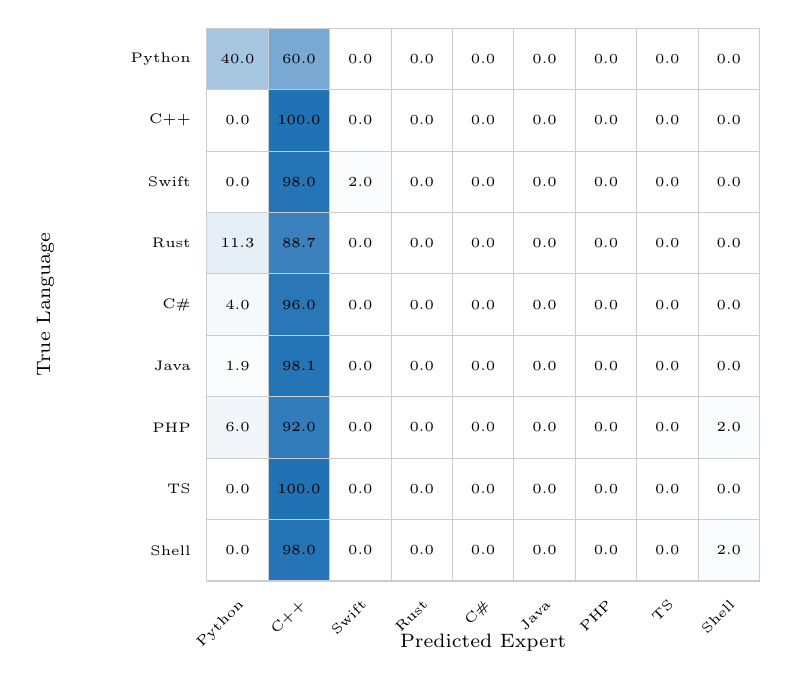
\begin{tikzpicture}
  \foreach \r/\c/\v in {
    0/0/40.0, 0/1/60.0, 0/2/0.0, 0/3/0.0, 0/4/0.0, 0/5/0.0, 0/6/0.0, 0/7/0.0, 0/8/0.0,
    1/0/0.0,  1/1/100.0,1/2/0.0, 1/3/0.0, 1/4/0.0, 1/5/0.0, 1/6/0.0, 1/7/0.0, 1/8/0.0,
    2/0/0.0,  2/1/98.0, 2/2/2.0, 2/3/0.0, 2/4/0.0, 2/5/0.0, 2/6/0.0, 2/7/0.0, 2/8/0.0,
    3/0/11.3, 3/1/88.7, 3/2/0.0, 3/3/0.0, 3/4/0.0, 3/5/0.0, 3/6/0.0, 3/7/0.0, 3/8/0.0,
    4/0/4.0,  4/1/96.0, 4/2/0.0, 4/3/0.0, 4/4/0.0, 4/5/0.0, 4/6/0.0, 4/7/0.0, 4/8/0.0,
    5/0/1.9,  5/1/98.1, 5/2/0.0, 5/3/0.0, 5/4/0.0, 5/5/0.0, 5/6/0.0, 5/7/0.0, 5/8/0.0,
    6/0/6.0,  6/1/92.0, 6/2/0.0, 6/3/0.0, 6/4/0.0, 6/5/0.0, 6/6/0.0, 6/7/0.0, 6/8/2.0,
    7/0/0.0,  7/1/100.0,7/2/0.0, 7/3/0.0, 7/4/0.0, 7/5/0.0, 7/6/0.0, 7/7/0.0, 7/8/0.0,
    8/0/0.0,  8/1/98.0, 8/2/0.0, 8/3/0.0, 8/4/0.0, 8/5/0.0, 8/6/0.0, 8/7/0.0, 8/8/2.0%
  } {
    \fill[heatblue!\v!white]
      ({\c*\EXcs}, {-\r*\EXcs}) rectangle ({(\c+1)*\EXcs}, {-(\r+1)*\EXcs});
    \node[font=\tiny] at ({(\c+0.5)*\EXcs}, {-(\r+0.5)*\EXcs}) {\v};
  }
  \draw[gray!40, thin] (0,0) grid[xstep=\EXcs, ystep=\EXcs] ({9*\EXcs},{-9*\EXcs});
  \foreach \c/\lbl in {0/Python, 1/C++, 2/Swift, 3/Rust, 4/C\#, 5/Java, 6/PHP, 7/TS, 8/Shell} {
    \node[font=\tiny, anchor=north east, rotate=45]
      at ({(\c+0.5)*\EXcs}, {-9*\EXcs-0.05}) {\lbl};
  }
  \foreach \r/\lbl in {0/Python, 1/C++, 2/Swift, 3/Rust, 4/C\#, 5/Java, 6/PHP, 7/TS, 8/Shell} {
    \node[font=\tiny, anchor=east]
      at ({-0.08}, {-(\r+0.5)*\EXcs}) {\lbl};
  }
  \node[font=\scriptsize] at ({4.5*\EXcs}, {-10.0*\EXcs}) {Predicted Expert};
  \node[font=\scriptsize, rotate=90, anchor=center] at (-2.05, {-4.5*\EXcs}) {True Language};
\end{tikzpicture}
\caption{Hard-routing confusion matrix (\%) of the \emph{instruction} router on the executable benchmark at the final training step. The C++ column dominates, collecting most mass from every language.}
\label{fig:confusion_exec}
\end{figure}

Despite this, GMM-Router still reaches 34.40\% Pass@1 (Table~\ref{tab:exec_avg}), because Round-1 uses soft, not hard, routing: the softmax at $\tau=1.0$ distributes weight across every fitted expert, so even when the C++ GMM has the highest log-likelihood, other experts receive non-negligible weight, and the language expert that genuinely models the target can still dominate the merged generation. This effect is most visible for TypeScript, which has 0\% hard-routing accuracy yet reaches 92.80\% Pass@1 --- close to the LoRA-per-task upper bound (93.20\%) --- indicating that soft mixing across experts approximates the dedicated TypeScript adapter closely.

Figure~\ref{fig:confusion_tb} shows the traceback router's confusion matrix, fitted on error tracebacks from failed Round-1 candidates rather than on instructions. The contrast is striking: average accuracy rises from 15.8\% to 96.8\%, with every language at or above 91.0\%. This gap is explained by the information content of error messages: unlike instruction prompts, which share vocabulary across languages, error tracebacks carry language-specific identifiers (Python's \texttt{AttributeError}/\texttt{TypeError}; Java's \texttt{NullPointerException}; C++ segmentation faults and template-instantiation errors; Swift's distinctively annotated memory-access violations), letting the traceback GMM learn well-separated per-language regions where the instruction GMM cannot. The dominant off-diagonal direction is toward Shell (6.0--8.0\% of Python and C++ samples), consistent with Shell capturing systems-level patterns --- command execution, file-system access, subprocess and environment handling --- that also occur in general-purpose languages.

\begin{figure}[t]
\centering
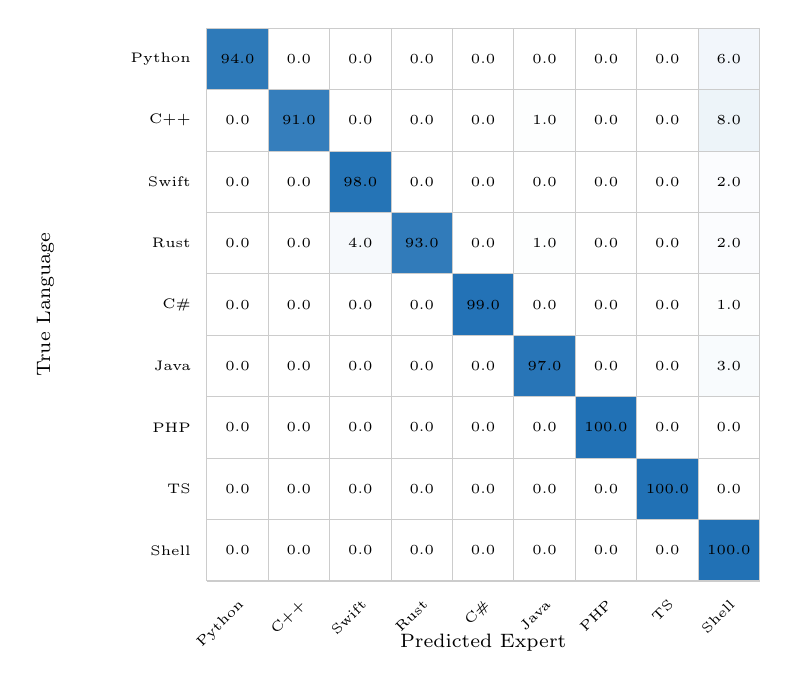
\begin{tikzpicture}
  \foreach \r/\c/\v in {
    0/0/94.0, 0/1/0.0,  0/2/0.0,  0/3/0.0,  0/4/0.0,  0/5/0.0,  0/6/0.0,   0/7/0.0,   0/8/6.0,
    1/0/0.0,  1/1/91.0, 1/2/0.0,  1/3/0.0,  1/4/0.0,  1/5/1.0,  1/6/0.0,   1/7/0.0,   1/8/8.0,
    2/0/0.0,  2/1/0.0,  2/2/98.0, 2/3/0.0,  2/4/0.0,  2/5/0.0,  2/6/0.0,   2/7/0.0,   2/8/2.0,
    3/0/0.0,  3/1/0.0,  3/2/4.0,  3/3/93.0, 3/4/0.0,  3/5/1.0,  3/6/0.0,   3/7/0.0,   3/8/2.0,
    4/0/0.0,  4/1/0.0,  4/2/0.0,  4/3/0.0,  4/4/99.0, 4/5/0.0,  4/6/0.0,   4/7/0.0,   4/8/1.0,
    5/0/0.0,  5/1/0.0,  5/2/0.0,  5/3/0.0,  5/4/0.0,  5/5/97.0, 5/6/0.0,   5/7/0.0,   5/8/3.0,
    6/0/0.0,  6/1/0.0,  6/2/0.0,  6/3/0.0,  6/4/0.0,  6/5/0.0,  6/6/100.0, 6/7/0.0,   6/8/0.0,
    7/0/0.0,  7/1/0.0,  7/2/0.0,  7/3/0.0,  7/4/0.0,  7/5/0.0,  7/6/0.0,   7/7/100.0, 7/8/0.0,
    8/0/0.0,  8/1/0.0,  8/2/0.0,  8/3/0.0,  8/4/0.0,  8/5/0.0,  8/6/0.0,   8/7/0.0,   8/8/100.0%
  } {
    \fill[heatblue!\v!white]
      ({\c*\EXcs}, {-\r*\EXcs}) rectangle ({(\c+1)*\EXcs}, {-(\r+1)*\EXcs});
    \node[font=\tiny] at ({(\c+0.5)*\EXcs}, {-(\r+0.5)*\EXcs}) {\v};
  }
  \draw[gray!40, thin] (0,0) grid[xstep=\EXcs, ystep=\EXcs] ({9*\EXcs},{-9*\EXcs});
  \foreach \c/\lbl in {0/Python, 1/C++, 2/Swift, 3/Rust, 4/C\#, 5/Java, 6/PHP, 7/TS, 8/Shell} {
    \node[font=\tiny, anchor=north east, rotate=45]
      at ({(\c+0.5)*\EXcs}, {-9*\EXcs-0.05}) {\lbl};
  }
  \foreach \r/\lbl in {0/Python, 1/C++, 2/Swift, 3/Rust, 4/C\#, 5/Java, 6/PHP, 7/TS, 8/Shell} {
    \node[font=\tiny, anchor=east]
      at ({-0.08}, {-(\r+0.5)*\EXcs}) {\lbl};
  }
  \node[font=\scriptsize] at ({4.5*\EXcs}, {-10.0*\EXcs}) {Predicted Expert};
  \node[font=\scriptsize, rotate=90, anchor=center] at (-2.05, {-4.5*\EXcs}) {True Language};
\end{tikzpicture}
\caption{Hard-routing confusion matrix (\%) of the \emph{traceback} router on the executable benchmark at the final training step. The strong diagonal contrasts sharply with Figure~\ref{fig:confusion_exec}.}
\label{fig:confusion_tb}
\end{figure}

\subsubsection{Knowledge transfer and forgetting dynamics}
\label{sec:forgetting}

This subsection evaluates GMM-Router, O-LoRA, SeqLoRA, and TreeLoRA --- the four methods with complete per-step evaluation matrices --- using BWT, FM, and FWT (Eqs.~\eqref{eq:fm}--\eqref{eq:bwt_fwt}).

\paragraph{CodeTask benchmark.} Table~\ref{tab:bwt_codetask} shows that GMM-Router achieves by far the lowest forgetting: BWT $-1.01\%$ and FM $1.01\%$, more than ten times smaller in magnitude than the next best, O-LoRA (BWT $-11.36\%$, FM $11.41\%$); SeqLoRA ($-22.10\%$) and TreeLoRA ($-33.79\%$) forget increasingly severely. All four methods show large, broadly comparable FWT ($+37.80\%$ to $+43.90\%$), indicating each learns each new task well on first exposure. GMM-Router's low forgetting follows directly from per-task expert isolation: later training never modifies an earlier expert's LoRA parameters or its already-fitted GMM component. The only residual source of forgetting is routing drift, since adding new GMM components shifts the relative log-posterior of each expert, occasionally reducing the weight an earlier-task input receives on its own expert even though neither its adapter nor its GMM has changed. Figure~\ref{fig:forgetting_concode} illustrates this: GMM-Router's retained CONCODE score declines only from $36.39\%$ at its peak to $35.06\%$ at the final step, while O-LoRA and SeqLoRA show sharp collapses with partial recovery, and TreeLoRA collapses from $36.80\%$ to near zero after the first subsequent task and never recovers.

\begin{table}[t]
\centering
\caption{BWT, FM, and FWT (\%) on the CodeTask benchmark. Negative BWT indicates net forgetting; lower FM is better; higher FWT indicates stronger in-task learning.}
\label{tab:bwt_codetask}
\small
\begin{tabular}{lccc}
\toprule
Method & BWT (\%) $\uparrow$ & FM (\%) $\downarrow$ & FWT (\%) $\uparrow$ \\
\midrule
\textbf{GMM-Router} & $-1.01$ & $1.01$ & $+37.80$ \\
O-LoRA     & $-11.36$ & $11.41$ & $+37.97$ \\
SeqLoRA    & $-22.10$ & $22.10$ & $+39.79$ \\
TreeLoRA   & $-33.79$ & $33.79$ & $+43.90$ \\
\bottomrule
\end{tabular}
\end{table}

\begin{figure}[t]
\centering
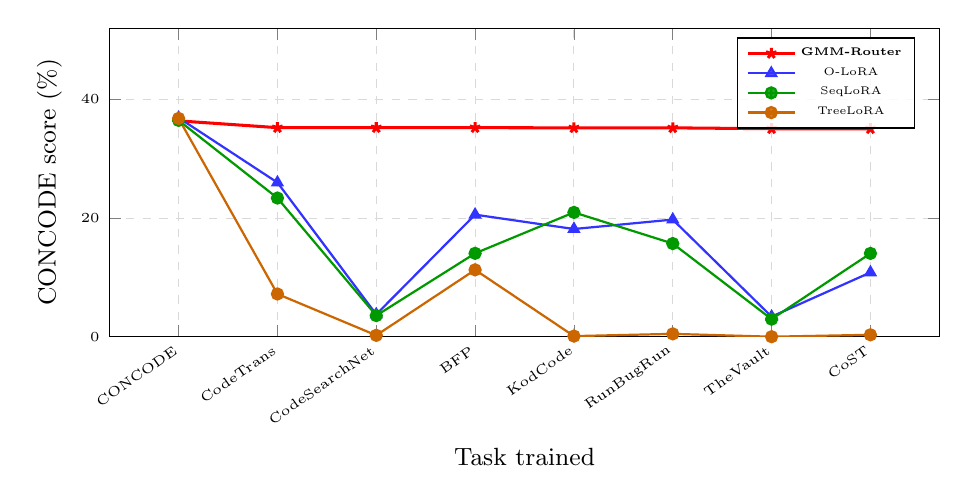
\begin{tikzpicture}
\begin{axis}[
    width=\linewidth, height=5.5cm,
    xlabel={Task trained},
    ylabel={CONCODE score (\%)},
    xtick={0,1,2,3,4,5,6,7},
    xticklabels={CONCODE,CodeTrans,CodeSearchNet,BFP,KodCode,RunBugRun,TheVault,CoST},
    xticklabel style={rotate=35, anchor=east, font=\tiny, yshift=-3pt},
    ymin=0, ymax=52,
    grid=major,
    grid style={dashed, gray!30},
    legend pos=north east,
    legend style={font=\tiny, nodes={scale=0.8}, draw=black, fill=white, fill opacity=0.85, text opacity=1},
    tick label style={font=\tiny},
    label style={font=\small},
]
\addplot[color=red, mark=star, thick, line width=1.1pt]
    coordinates {(0,36.39)(1,35.24)(2,35.24)(3,35.24)(4,35.21)(5,35.21)(6,35.06)(7,35.06)};
\addlegendentry{\textbf{GMM-Router}}
\addplot[color=blue!80, mark=triangle*, thick]
    coordinates {(0,36.91)(1,25.99)(2,3.77)(3,20.58)(4,18.16)(5,19.75)(6,3.39)(7,10.84)};
\addlegendentry{O-LoRA}
\addplot[color=green!60!black, mark=oplus*, thick]
    coordinates {(0,36.47)(1,23.38)(2,3.57)(3,14.06)(4,20.96)(5,15.71)(6,2.97)(7,14.05)};
\addlegendentry{SeqLoRA}
\addplot[color=orange!80!black, mark=otimes*, thick]
    coordinates {(0,36.80)(1,7.21)(2,0.24)(3,11.28)(4,0.11)(5,0.49)(6,0.01)(7,0.33)};
\addlegendentry{TreeLoRA}
\end{axis}
\end{tikzpicture}
\caption{Retained CONCODE score after each task in the CodeTask sequence. GMM-Router remains nearly flat ($36.39\%\to35.06\%$); O-LoRA and SeqLoRA show severe drops with partial recovery; TreeLoRA suffers substantial catastrophic forgetting.}
\label{fig:forgetting_concode}
\end{figure}

\paragraph{Executable benchmark.} Table~\ref{tab:bwt_exec} shows a different pattern. GMM-Router and O-LoRA show negative BWT on both Pass@1 and Pass@5, indicating net forgetting, because the instruction router's GMM boundaries shift as later language experts are added, and this drift is more pronounced here than on CodeTask since all nine languages share deep syntactic overlap, so their GMM regions sit close together and a new language's GMM displaces boundaries more than in the type-diverse CodeTask sequence. SeqLoRA and TreeLoRA instead show positive BWT, benefiting directly from cross-language reinforcement in their shared parameters. On FM, GMM-Router is competitive on Pass@1 ($1.77\%$, versus O-LoRA's $1.62\%$) and lowest on Pass@5 ($3.83\%$): because each adapter is frozen after training, no single later step can catastrophically overwrite it, so forgetting accumulates gradually through routing drift rather than through parameter overwriting, keeping worst-case single-step drops small; SeqLoRA and TreeLoRA show the opposite trade-off, with positive BWT but much higher FM ($6.92\%$ and $6.38\%$ Pass@1). All four methods show large FWT, and GMM-Router leads on Pass@5 FWT ($+25.97\%$) because each language adapter trains exclusively on its own data without competing gradients from other languages in a shared parameter space, fitting the target distribution more tightly than shared-parameter methods must. Swift illustrates the isolation guarantee directly: GMM-Router's retained Swift Pass@1 starts and ends the remaining eight-task sequence at exactly $66.40\%$ (dipping to $63.20\%$ at one intermediate step before returning), whereas TreeLoRA erodes by $2.4$pp and O-LoRA/SeqLoRA start lower but rise through cross-language reinforcement.

\begin{table}[t]
\centering
\caption{BWT, FM, and FWT (\%) on the executable benchmark. Positive BWT indicates backward enhancement; lower FM is better; higher FWT indicates stronger in-task learning.}
\label{tab:bwt_exec}
\scriptsize
\resizebox{\linewidth}{!}{%
\begin{tabular}{lcccccc}
\toprule
\multirow{2}{*}{Method} & \multicolumn{2}{c}{BWT $\uparrow$} & \multicolumn{2}{c}{FM $\downarrow$} & \multicolumn{2}{c}{FWT $\uparrow$} \\
\cmidrule(lr){2-3}\cmidrule(lr){4-5}\cmidrule(lr){6-7}
 & P@1 (\%) & P@5 (\%) & P@1 (\%) & P@5 (\%) & P@1 (\%) & P@5 (\%) \\
\midrule
\textbf{GMM-Router} & $-1.22$ & $-2.61$ & $1.77$ & $3.83$ & $+20.94$ & $+25.97$ \\
O-LoRA     & $-0.59$ & $-1.36$ & $1.62$ & $4.51$ & $+19.61$ & $+18.85$ \\
SeqLoRA    & $+0.88$ & $+0.28$ & $6.92$ & $10.47$ & $+22.07$ & $+20.99$ \\
TreeLoRA   & $+1.67$ & $+3.68$ & $6.38$ & $8.44$ & $+21.08$ & $+18.63$ \\
\bottomrule
\end{tabular}%
}
\end{table}

Taken together, RQ3 shows a clear cross-benchmark contrast: on the diverse CodeTask sequence, per-expert isolation reduces net forgetting by more than an order of magnitude relative to the best shared-parameter baseline; on the homogeneous executable benchmark, routing drift from closely packed language GMMs causes mild net forgetting, but GMM-Router still keeps FM competitive and leads on Pass@5 FWT.

\subsection{RQ4: Iterative refinement}
\label{sec:refinement}

GMM-Router's Round-2 pipeline (Section~\ref{sec:traceback}) triggers only for samples where all five Round-1 candidates fail. Table~\ref{tab:ablation_refinement} ablates its two components: the traceback router with JSD-gated combination, and an optional adapter-refinement step.

\begin{table}[t]
\centering
\caption{Ablation of Round-2 pipeline components on the executable benchmark. Best averages in bold.}
\label{tab:ablation_refinement}
\small
\resizebox{\linewidth}{!}{%
\begin{tabular}{lcc}
\toprule
Configuration & Avg.\ Pass@1 (\%) & Avg.\ Pass@5 (\%) \\
\midrule
Round-1 only & 33.04 & 41.66 \\
Round-2, original adapter + JSD & \textbf{34.40} & \textbf{47.75} \\
Round-2, refined adapter + JSD & 33.62 & 43.97 \\
\bottomrule
\end{tabular}%
}
\end{table}

Adding Round-2 with the original adapter and JSD-gated combination raises average Pass@1 by $1.36$pp ($33.04\%\to34.40\%$) and Pass@5 by $6.09$ points ($41.66\%\to47.75\%$), concentrated on Rust ($+9.05\%$ Pass@1, $+39.62\%$ Pass@5) and Java ($+2.65\%$ Pass@1, $+13.18\%$ Pass@5), the two languages where Round-1 candidates most often exhaust all five attempts. Table~\ref{tab:r2_lang} breaks Round-2 coverage (fraction of samples triggering Round-2) and lift (fraction of triggered samples recovered) down by language at the final training step.

\begin{table}[t]
\centering
\caption{Round-2 coverage and lift per language at the final training step. Languages sorted by lift, descending.}
\label{tab:r2_lang}
\small
\begin{tabular}{lrrr}
\toprule
Language   & Coverage (\%) & Triggered/Total & Lift (\%) \\
\midrule
Rust       & 81.1 & 43/53 & 48.8 \\
Java       & 67.9 & 36/53 & 19.4 \\
Shell      & 64.0 & 32/50 &  3.1 \\
C++        & 92.0 & 46/50 &  0.0 \\
C\#        & 92.0 & 46/50 &  0.0 \\
Python     & 54.0 & 27/50 &  0.0 \\
PHP        & 54.0 & 27/50 &  0.0 \\
Swift      & 20.0 & 10/50 &  0.0 \\
TypeScript &  0.0 &  0/50 & --- \\
\bottomrule
\end{tabular}
\end{table}

C++ and C\# both trigger Round-2 on 92\% of their test samples yet achieve zero lift: their failures stem from generation quality rather than routing mismatch, so redirecting to a different expert does not help. TypeScript never triggers Round-2 because every Round-1 candidate already passes, consistent with its near-perfect Table~\ref{tab:exec_p1}/\ref{tab:exec_p5} scores. Refining each adapter on error-repair pairs (Table~\ref{tab:ablation_refinement}, third row) gives a mixed picture: Java Pass@5 rises further (to $47.17\%$), but Rust declines markedly ($58.49\%\to24.53\%$ Pass@5), likely because repair targets are drawn from any passing candidate rather than one that specifically addresses the traceback shown, so the refined adapter can be trained on a repair signal that is not causally linked to the reported error (Section~\ref{sec:limitations}).

Table~\ref{tab:jsd_summary} isolates the Round-2 routing rule itself, holding the original (non-refined) adapters fixed and comparing traceback-alone routing, an unweighted sum of instruction and traceback log-posteriors, and the JSD-gated combination of Eq.~\eqref{eq:jsd_gated}.

\begin{table}[t]
\centering
\caption{Average Pass@1/Pass@5 (\%) under four Round-2 routing strategies (original adapters).}
\label{tab:jsd_summary}
\small
\begin{tabular}{lcc}
\toprule
Configuration & Avg.\ Pass@1 (\%) & Avg.\ Pass@5 (\%) \\
\midrule
Round-1 only               & 33.04 & 41.66 \\
Traceback alone            & 34.13 & 46.48 \\
Unweighted sum              & 34.13 & 46.48 \\
\textbf{JSD-gated}          & \textbf{34.40} & \textbf{47.75} \\
\bottomrule
\end{tabular}
\end{table}

Traceback routing is the primary driver of Round-2 gains: moving from Round-1 to any Round-2 variant, Rust improves most (Pass@1 $10.57\%\to19.62\%$, Pass@5 $18.87\%\to58.49\%$), since Rust's distinctive borrow-checker and lifetime diagnostics let the traceback GMM identify and redirect these failures regardless of how the instruction router scored the problem; six of the nine languages show no change across Round-2 variants because their Round-1 candidates either already pass (TypeScript) or fail in ways rerouting cannot fix (C++, C\#, Python, PHP, Swift). The unweighted sum produces results identical to traceback alone across all languages, because on samples that already exhausted five Round-1 attempts the traceback GMM assigns much sharper posterior mass to a single expert than the instruction GMM does, so summing the two log-posteriors does not change the top-ranked expert. JSD gating is what recovers the remaining conflicted samples: it behaves like the combined posterior when the two routers agree and blends toward uniform when they conflict, which prevents overconfident misrouting and lifts Java (Pass@5 $35.85\%\to45.28\%$, $+9.43$pp; Pass@1 $+1.89$pp) and Shell (Pass@5 $+2$pp) beyond what traceback-alone or the unweighted sum achieve; Rust is unaffected because the traceback router alone already accounts for most of its gain.

\subsection{Discussion}
\label{sec:discussion}

\subsubsection{Cross-benchmark comparison}
\label{sec:crossbench}

Figure~\ref{fig:method_comparison} plots each method's CodeTask average against its executable Pass@1, exposing a tension among the baselines: methods that maximize executable Pass@1 through parameter or gradient sharing (SeqLoRA, TreeLoRA) forget on the diverse CodeTask sequence, while methods that isolate tasks to protect CodeTask performance (O-LoRA, Online-CL-LLM) lack a dedicated task-agnostic routing mechanism and only reach moderate executable Pass@1. GMM-Router occupies a distinct position: $51.62\%$ on CodeTask --- $8.85$pp above O-LoRA and $16.72$pp above SeqLoRA --- while its $34.40\%$ executable Pass@1 exceeds the non-iterative upper bound, and its $47.75\%$ Pass@5 leads all methods. This is consistent with per-task expert isolation and soft distribution-level routing being complementary: isolation prevents forgetting on diverse sequences, while soft routing and iterative refinement provide candidate diversity and recovery on homogeneous ones.

\begin{figure}[t]
\centering
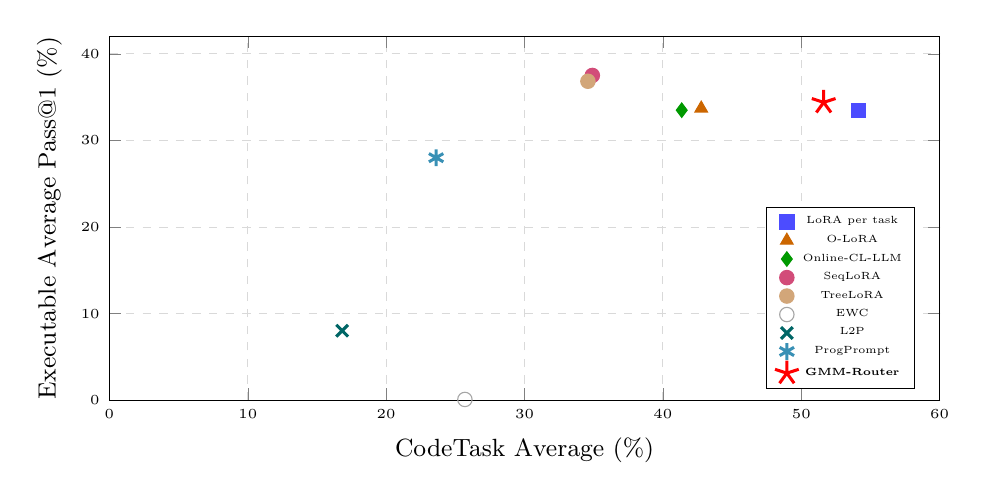
\begin{tikzpicture}
\begin{axis}[
    width=\linewidth, height=6.2cm,
    xlabel={CodeTask Average (\%)},
    ylabel={Executable Average Pass@1 (\%)},
    xmin=0, xmax=60,
    ymin=0, ymax=42,
    grid=major,
    grid style={dashed, gray!30},
    legend pos=south east,
    legend style={font=\tiny, nodes={scale=0.75}, draw=black},
    tick label style={font=\tiny},
    label style={font=\small},
]
\addplot[only marks, mark=square*, mark size=2.6pt, color=blue!70]
    coordinates {(54.15, 33.46)};
\addlegendentry{LoRA per task}
\addplot[only marks, mark=triangle*, mark size=2.6pt, color=orange!80!black]
    coordinates {(42.77, 33.71)};
\addlegendentry{O-LoRA}
\addplot[only marks, mark=diamond*, mark size=2.6pt, color=green!60!black]
    coordinates {(41.36, 33.50)};
\addlegendentry{Online-CL-LLM}
\addplot[only marks, mark=oplus*, mark size=2.6pt, color=purple!70]
    coordinates {(34.90, 37.51)};
\addlegendentry{SeqLoRA}
\addplot[only marks, mark=otimes*, mark size=2.6pt, color=brown!70]
    coordinates {(34.58, 36.84)};
\addlegendentry{TreeLoRA}
\addplot[only marks, mark=o, mark size=2.6pt, color=gray!70]
    coordinates {(25.69, 0.09)};
\addlegendentry{EWC}
\addplot[only marks, mark=x, mark size=3pt, color=teal!80!black, line width=1.1pt]
    coordinates {(16.82, 8.03)};
\addlegendentry{L2P}
\addplot[only marks, mark=asterisk, mark size=3pt, color=cyan!70!black, line width=1.1pt]
    coordinates {(23.61, 28.01)};
\addlegendentry{ProgPrompt}
\addplot[only marks, mark=star, mark size=4.5pt, color=red, line width=1.1pt]
    coordinates {(51.62, 34.40)};
\addlegendentry{\textbf{GMM-Router}}
\end{axis}
\end{tikzpicture}
\caption{CodeTask average (\%) vs.\ executable average Pass@1 (\%) for each method. LoRA per task is the upper bound. Methods in the upper-right corner are preferred; methods that trade one benchmark for the other appear off-diagonal.}
\label{fig:method_comparison}
\end{figure}

\subsubsection{Qualitative example: Round-2 recovery via traceback routing}
\label{sec:error_analysis}

The following case illustrates why the traceback router recovers samples the instruction router cannot. For a Rust task (implementing \texttt{is\_arithmetic\_sequence}), the instruction router assigns $\alpha_{\text{cpp}}=1.0$ with zero weight elsewhere, and all five Round-1 candidates fail to compile with \texttt{error[E0601]: `main` function not found}: the C++-trained adapter generates a bare function body following the C++ submission convention, where the harness supplies its own entry point, but Rust requires an explicit \texttt{fn main()} to compile as a standalone binary regardless of whether the function logic is correct. In Round-2, the traceback GMM redistributes routing weight to $\alpha_{\text{rust}}=0.384$ (Figure~\ref{fig:case_routing}), because \texttt{error[E0601]} is a diagnostic vocabulary specific to Rust's compilation model and absent from C++ output. The regenerated candidate is functionally identical to the Round-1 output except for the addition of \texttt{fn main()}, which the Rust adapter produces because its training data includes the standalone-binary scaffold. This example is representative of the pattern behind Table~\ref{tab:r2_lang}: the instruction GMM fails when generic problem phrasing makes two languages indistinguishable at the embedding level, while the traceback GMM succeeds because compilation errors are intrinsically language-specific diagnostics.

\begin{figure}[t]
\centering
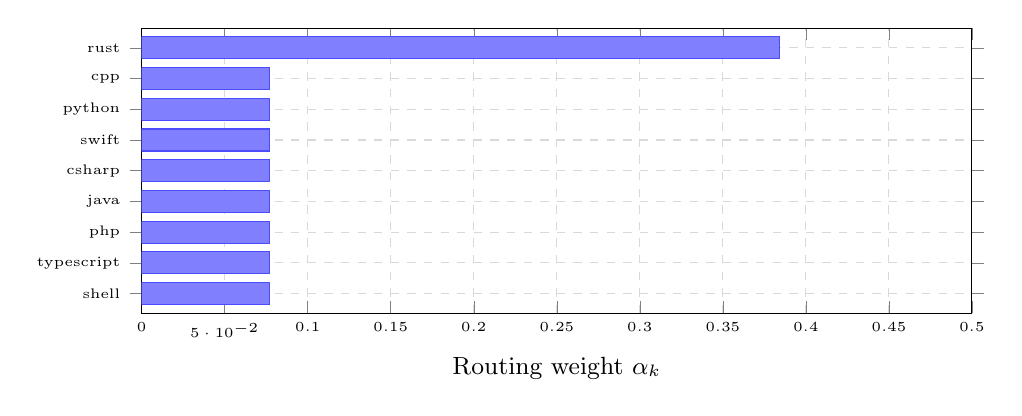
\begin{tikzpicture}
\begin{axis}[
    xbar, bar width=0.28cm,
    width=\linewidth, height=5.2cm,
    symbolic y coords={shell,typescript,php,java,csharp,swift,python,cpp,rust},
    ytick=data,
    xlabel={Routing weight $\alpha_k$},
    xmin=0, xmax=0.5,
    grid=major,
    grid style={dashed, gray!30},
    tick label style={font=\tiny},
    label style={font=\small},
    enlarge y limits=0.08,
]
\addplot[fill=blue!50, draw=blue!70]
    coordinates {
        (0.3839,rust) (0.0770,cpp)   (0.0770,python)
        (0.0770,swift) (0.0770,csharp) (0.0770,java)
        (0.0770,php)  (0.0770,typescript) (0.0770,shell)
    };
\end{axis}
\end{tikzpicture}
\caption{Round-2 routing weights $\alpha_k$ after traceback-GMM redistribution for the example in Section~\ref{sec:error_analysis}. The Rust expert rises from $0$ to $0.384$; the remaining weight spreads approximately evenly across the other eight experts.}
\label{fig:case_routing}
\end{figure}

\subsubsection{Limitations and threats to validity}
\label{sec:limitations}

\textbf{Construct validity.} BLEU and CodeBLEU, used on the CodeTask benchmark, cannot fully distinguish functionally correct code from code that merely resembles a reference (Section~\ref{sec:metrics}); this is mitigated by the executable benchmark's unit-test grading, but the two tracks are not directly comparable and are reported separately throughout.

\textbf{Internal validity.} All continual learning metrics (Eqs.~\eqref{eq:fm}--\eqref{eq:bwt_fwt}) depend on the fixed task order used during training (Section~\ref{sec:hyperparams}); a different order could change which tasks interfere with which, particularly on the executable benchmark where routing drift is order-dependent (Section~\ref{sec:forgetting}). The repair pairs used for adapter refinement (Section~\ref{sec:traceback}) pair a failed candidate's traceback with any passing candidate rather than one verified to resolve that specific error, which is a plausible explanation for the Rust regression in Table~\ref{tab:ablation_refinement} and is a limitation of the training signal rather than of the routing mechanism itself.

\textbf{External validity.} Experiments use a single 1.5B-parameter backbone (Section~\ref{sec:baselines}); routing behavior --- particularly the C++ attractor effect in Figure~\ref{fig:confusion_exec} --- may differ for backbones with different pretraining data or scale. The executable benchmark's test set is drawn from McEval and capped at 50--53 problems per language (Table~\ref{tab:exec_stats}), which bounds the precision of the per-language Pass@$k$ estimates in Tables~\ref{tab:exec_p1}--\ref{tab:exec_p5}.

\textbf{Conclusion validity.} Per-task expert isolation, while effective at preventing forgetting, limits transfer between related tasks; this is most visible on C\# and Rust in the executable benchmark (Section~\ref{sec:perlang}), where shared-adaptation baselines benefit from cross-language transfer that GMM-Router cannot replicate without an explicit sharing mechanism. Routing quality also depends on how well the frozen backbone separates task distributions at the chosen layer $\ell^*$; tasks with similar surface-level inputs but different output objectives, such as the nine syntactically related programming languages, are intrinsically harder to separate by density estimation alone (Section~\ref{sec:routing_analysis}). Finally, adapter storage grows linearly with the number of tasks, which may become a practical constraint on much longer task sequences than the eight- and nine-task streams studied here.

\section{Related Work}
\label{sec:related_work}

\subsection{Continual learning methods}
\label{sec:rw_cl}

\textbf{Regularization-based methods} reduce forgetting by penalizing changes to parameters considered important for earlier tasks, without allocating separate modules per task. EWC \citep{kirkpatrick2017overcoming} estimates parameter importance from the Fisher information matrix and penalizes deviation from previous values; Learning without Forgetting \citep{li2017learning} instead preserves the model's output distribution via knowledge distillation; Synaptic Intelligence \citep{zenke2017continual} and Memory Aware Synapses \citep{aljundi2018memory} accumulate importance online. These methods are memory-efficient because they require no replay buffer, but because all tasks share one parameter space, their protection weakens as the number and diversity of tasks grows, which Table~\ref{tab:codetask_qwen} confirms for EWC on the eight-task CodeTask sequence. GMM-Router sidesteps this failure mode by allocating a dedicated LoRA adapter per task (Section~\ref{sec:experts}) rather than sharing one regularized parameter set.

\textbf{Memory-based methods} store information from earlier tasks and replay it during later training. GEM and A-GEM \citep{lopezpaz2017gem,chaudhry2019agem} use stored examples to constrain gradients so earlier tasks are not harmed; DER++ \citep{buzzega2020dark} replays stored logits to match past model behavior; Deep Generative Replay \citep{shin2017continual} generates pseudo-examples instead of storing real ones. These are strong baselines but increase per-step cost and conflict with settings, such as proprietary or privacy-sensitive code repositories, where retaining historical data is undesirable (Section~\ref{sec:motivation}). GMM-Router requires no stored training examples at inference time: its GMMs are fitted once from task-level routing embeddings during training and then frozen.

\textbf{Architecture-based methods} handle forgetting by partitioning model capacity across tasks. Progressive Neural Networks add a branch per task, PackNet reuses a fixed network through pruning, and HAT learns hard attention masks \citep{rusu2016progressive,mallya2018packnet,serra2018overcoming}; L2P \citep{wang2022learning} learns a shared, dynamically retrieved prompt pool, and Progressive Prompts \citep{razdaibiedina2023progressive} keeps earlier prompts fixed while adding new ones per task. These are included as baselines in Section~\ref{sec:baselines} (L2P, ProgPrompt); their limited representational capacity relative to full LoRA experts is consistent with their weaker CodeTask and executable-benchmark results (Tables~\ref{tab:codetask_qwen}--\ref{tab:exec_avg}).

\textbf{LoRA-based continual learning} is the branch most directly related to GMM-Router. A single LoRA trained sequentially (SeqLoRA in this paper) keeps storage flat but allows forgetting because all tasks share the same low-rank update \citep{hu2022lora}; per-task LoRAs (the LoRA-per-task upper bound) prevent forgetting but require storage that grows linearly and either task identity or a router at inference. O-LoRA \citep{wang2023orthogonal} reduces interference by learning task updates in mutually orthogonal low-rank subspaces; GORP \citep{wang2025continual} uses low-rank gradient projection to expand the optimization space; TreeLoRA \citep{qian2025treelora} organizes adapters hierarchically by gradient similarity. CoLoR \citep{wistuba2023continual} studies whether LoRA itself is an effective continual learning mechanism for pretrained transformers; C-LoRA \citep{zhang2025clora} introduces a learnable routing matrix that manages low-rank updates across tasks while encouraging orthogonality; CL-LoRA \citep{he2025cllora} combines task-shared and task-specific adapters with orthogonal structures and distillation for rehearsal-free continual learning. These methods reduce --- but, because they still couple tasks through a partially shared subspace, do not eliminate --- cross-task interference, and the number of usable orthogonal directions shrinks as more tasks are added (Section~\ref{sec:introduction}). GMM-Router instead removes coupling between adapters entirely by isolating each task in its own LoRA module and coordinating them only at inference, through routing rather than through a shared or orthogonalized subspace.

Online-CL-LLM \citep{cheng2025exploiting}, evaluated as a baseline in Section~\ref{sec:baselines}, is the method closest in spirit to GMM-Router: it characterizes each PEFT block by a representative feature distribution and dynamically selects blocks per input without task labels, sharing GMM-Router's reliance on distributional information for task-agnostic routing. It differs in that it selects among existing PEFT blocks rather than combining them, whereas GMM-Router uses explicit per-task GMM posterior scores (Eq.~\eqref{eq:snorm}) to support both hard selection and soft, weight-level adapter merging (Eq.~\eqref{eq:weight_merge}), which Section~\ref{sec:exec_results} shows is responsible for GMM-Router's Pass@5 lead on the executable benchmark.

\subsection{Mixture of experts and density-based routing}
\label{sec:rw_moe}

The routing mechanism in Section~\ref{sec:methodology} is related to the mixture-of-experts literature, in which expert networks specialize in different parts of the input space and a gating function determines their contribution. \citet{jacobs1991adaptive} introduced adaptive mixtures of local experts with a learned gating network, and \citet{jordan1994hierarchical} extended this to hierarchical mixtures trained with EM-style learning, establishing that routing and expert specialization admit a principled probabilistic interpretation. In modern deep learning, sparsely-gated mixture-of-experts layers \citep{shazeer2017outrageously} and Switch Transformers \citep{fedus2022switch} activate only a small number of experts per input using learned neural gating rather than an explicit density model, but the underlying motivation --- routing different inputs to specialized modules --- is the same. GMM-Router differs from this line of work in two respects relevant to the continual setting: its gate is an explicit, per-task Gaussian Mixture Model fitted independently for each task as it arrives (Section~\ref{sec:router}), rather than a single jointly trained gating network that would need to be retrained as new experts are added; and its routing features are extracted from a frozen backbone through a fixed orthonormal projection (Section~\ref{sec:features}) specifically so that GMM densities fitted at different points in the task sequence remain comparable, a stability requirement that does not arise in the single-training-run setting where standard MoE gating is typically deployed.

\subsection{Code language models and evaluation}
\label{sec:rw_code}

Pretrained code language models, reviewed in Section~\ref{sec:clm_background}, provide the backbones on which all methods compared in this paper are built \citep{feng2020codebert,guo2021graphcodebert,guo2022unixcoder,ahmad2021plbart,wang2021codet5,wang2023codet5plus,fried2023incoder,roziere2023codellama,lozhkov2024starcoder2,hui2024qwen25coder}. Continual learning for this domain was introduced by CodeTask-CL \citep{yadav2023exploring}, which this paper extends from four to eight tasks (Section~\ref{sec:codetask_data}) because a four-task sequence scored only by BLEU \citep{papineni2002bleu} and CodeBLEU \citep{ren2020codebleu} under-represents both the length of realistic deployment sequences and the risk that text-similarity metrics reward superficially correct but functionally broken code. Execution-based evaluation, following the Codex/HumanEval methodology of \citet{chen2021evaluating} and the multilingual MultiPL-E benchmark \citep{cassano2023multipl}, addresses the second gap directly but has not previously been combined with sequential, task-agnostic continual learning; the executable benchmark and deduplication pipeline in Section~\ref{sec:data} are constructed specifically to close this gap.

\section{Conclusion and Future Work}
\label{sec:conclusion}

This paper studied task-agnostic, parameter-efficient continual learning for sequential code generation, a setting in which a model must adapt to a growing stream of generation, translation, summarization, refinement, and multilingual program-synthesis tasks without forgetting earlier ones and without access to task identity at inference time. We proposed GMM-Router, which trains a dedicated LoRA expert per task on a frozen backbone and routes each query using a diagonal Gaussian Mixture Model fitted on routing embeddings extracted through a fixed orthonormal projection, so that per-task density models remain comparable as the task sequence grows; for executable code generation, a second GMM fitted on runtime error tracebacks, combined with the instruction router through a Jensen--Shannon-divergence-gated rule, recovers samples that fail on every Round-1 attempt.

Across two complementary benchmarks --- an eight-task extension of CodeTask-CL scored by text-overlap metrics and a nine-language executable benchmark scored by unit-test execution --- the experiments in Section~\ref{sec:results} answer the four research questions posed in Section~\ref{sec:rqs}. GMM-Router achieves the highest average score (51.62\%) among all task-agnostic continual learning methods on CodeTask, approaching the task-identity upper bound (54.15\%) with near-zero forgetting (BWT $-1.01\%$, FM $1.01\%$; RQ1, RQ3). On the executable benchmark, it reaches 34.40\% Pass@1 and the highest Pass@5 (47.75\%) among all evaluated methods, exceeding the non-iterative upper bound on Pass@1 (RQ2). Router assignment analysis shows a sharp contrast between the two benchmarks: instruction-based hard routing reaches 90.6\% accuracy on the type-diverse CodeTask sequence but only 15.8\% on the syntactically homogeneous executable benchmark, where the complementary traceback router recovers 96.8\% accuracy in Round-2 (RQ3). The iterative refinement pipeline contributes 1.36pp Pass@1 and 6.09 points Pass@5 over Round-1 alone, concentrated on Rust and Java, and JSD gating specifically recovers Java and Shell beyond what traceback routing alone achieves (RQ4). Taken together, these results indicate that per-task expert isolation and density-based probabilistic routing are complementary: isolation prevents forgetting on structurally diverse task sequences, and soft, distribution-level routing with iterative refinement provides candidate diversity and error recovery on structurally homogeneous ones, without requiring task labels, data replay, or a shared adapter subspace.

GMM-Router also has limitations, discussed in Section~\ref{sec:limitations}, that motivate three directions for future work. First, per-task expert isolation limits knowledge transfer between related tasks, most visibly on C\# and Rust in the executable benchmark, where shared-adaptation baselines benefit from cross-language transfer that GMM-Router cannot currently exploit; a promising direction is a lightweight, jointly trained module shared beneath the task-specific adapter layers, or a distillation step between adapters for tasks whose GMMs the router already identifies as overlapping, turning the density model into a signal for both routing and selective knowledge consolidation. Second, adapter storage grows linearly with the number of tasks; dynamic expert merging --- pruning or merging adapters whose GMMs exhibit high overlap in the routing space --- or post-hoc adapter compression could keep GMM-Router practical for task sequences much longer than the eight- and nine-task streams studied here. Third, the repair pairs used for adapter refinement in Section~\ref{sec:refinement} do not guarantee that the target solution resolves the specific error shown in the accompanying traceback, which is a plausible cause of the Rust regression observed when refinement is combined with JSD-gated routing (Table~\ref{tab:ablation_refinement}); constructing repair pairs with execution-guided search for patches that provably fix the reported error is a natural next step and may recover Rust's gains while preserving the improvement already observed on Java.


\section*{Acknowledgments}
The author thanks Dr.\ Ngo Van Linh for supervision and feedback throughout this work, and Le Hai Nam for guidance on the direction and technical execution of the research. The author also thanks Nguyen Minh Tung and Cao Van Dong of the Foundation Models group at BKAI Laboratory for discussions and suggestions that improved this work, and Hanoi University of Science and Technology for the academic environment and computational resources that made this research possible.

\section*{Funding}
TODO: insert funding source or a statement that no specific funding was received.

\section*{Declaration of competing interest}
TODO: insert competing-interest declaration.

\section*{Data availability}
TODO: insert links to the released CodeTask extension, the executable benchmark splits, and the code implementing GMM-Router, or a statement of the conditions under which they will be made available.

\section*{Declaration of generative AI and AI-assisted technologies in the writing process}
During the preparation of this work, the author used an AI coding assistant (Claude, Anthropic) to help restructure and condense prior thesis material into this manuscript's Journal of Systems and Software format. The author reviewed and edited the resulting material and takes full responsibility for the content of the publication.

% Uncomment and use the natbib style already configured above.
\bibliographystyle{cas-model2-names}
\bibliography{refs}

\end{document}
